%%%%%%%%%%%%%%%%%%%%%%%%%%%%%%%%%%%%%%%%%%%%%%%%%%%%%%%%%%%%%%%%%%%%%%%%%%%%%%%%
% ISE Lab -- Topic
% Giovanni Ciatto
% Alma Mater Studiorum - Università di Bologna
% mailto:giovanni.ciatto@unibo.it
%%%%%%%%%%%%%%%%%%%%%%%%%%%%%%%%%%%%%%%%%%%%%%%%%%%%%%%%%%%%%%%%%%%%%%%%%%%%%%%%
%\documentclass[handout]{beamer}\mode<handout>{\usetheme{default}}
%
\documentclass[presentation]{beamer}\mode<presentation>{\usetheme{AMSBolognaFC}}
%\documentclass[handout]{beamer}\mode<handout>{\usetheme{AMSBolognaFC}}
%%%%%%%%%%%%%%%%%%%%%%%%%%%%%%%%%%%%%%%%%%%%%%%%%%%%%%%%%%%%%%%%%%%%%%%%%%%%%%%%
\usepackage{ise-lab-common}
\usepackage{ise-lab-ske}
% version
\newcommand{\versionmajor}{1}
\newcommand{\versionminor}{2}
\newcommand{\versionpatch}{1}
\newcommand{\version}{\versionmajor.\versionminor.\versionpatch}
%%%%%%%%%%%%%%%%%%%%%%%%%%%%%%%%%%%%%%%%%%%%%%%%%%%%%%%%%%%%%%%%%%%%%%%%%%%%%%%%
\title[\currentLab{} -- XAI via SKE]{
    eXplainable Artificial Intelligence via Symbolic Knowledge Extraction
}
%
\subtitle{\courseName{} / Module \moduleN{} (\courseAcronym)}
%
\author[\sspeaker{\gcShort}]{\speaker{\gcFull} \\ \gcEmail}
%
\institute[\disiShort, \uniboShort]{\disi{} (\disiShort)\\\unibo}
%
\date[A.Y. \academicYear{} (v.\ \version)]{Academic Year \academicYear{}\\(version \version)}
%
%%%%%%%%%%%%%%%%%%%%%%%%%%%%%%%%%%%%%%%%%%%%%%%%%%%%%%%%%%%%%%%%%%%%%%%%%%%%%%%%
\begin{document}
%%%%%%%%%%%%%%%%%%%%%%%%%%%%%%%%%%%%%%%%%%%%%%%%%%%%%%%%%%%%%%%%%%%%%%%%%%%%%%%%

%/////////
\frame{\titlepage}
%/////////

%%===============================================================================
\section*{Outline}
%%===============================================================================
%
%%/////////
\frame[c]{\tableofcontents[hideallsubsections]}
%%/////////

%===============================================================================
\section{Motivation \& Context}
%===============================================================================

\begin{frame}{Context}
    \begin{itemize}
        \item Pervasive \alert{adoption} of AI- and ML-powered solution world-wide
        %
        \begin{itemize}
            \item for \alert{automation} and decision support
        \end{itemize}
        
        \vfill
        
        \item[$\Rightarrow$] Several activities are (partially?) \alert{delegated} to intelligent machines
        %
        \begin{itemize}
            \item[!] even activities from critical domains: finance, health care, etc
        \end{itemize}
        
        \vfill
        
        \item Especially in ML, we let machines learn specific tasks from data
        %
        \begin{itemize}
            \item through the production of \alert{numeric} predictors, a.k.a. \alert{black-boxes}
            \item instead of programming such tasks ourselves
        \end{itemize}
        
        \vfill
        
        \item Unfortunately, black-boxes tend to be inherently
        %
        \begin{itemize}
            \item \alert{opaque} w.r.t. the knowledge they acquire from data\ccite{Lipton2018}
            \item \alert{sub-optimal} in performance as they are trained to minimise errors
        \end{itemize}
        
    \end{itemize}
\end{frame}

\begin{frame}[c]{Motivation}
    \alert{Opaqueness} of ML-based predictors brings several \alert{drawbacks}\ccite{guidotti2018survey,Lipton2018}:
    %
    \vfill
    %
    \begin{itemize}
        \item difficulty in \alert{understanding} what a black-box has learned from data
        %
        \begin{itemize}
            \item[e.g.] ``snowy background'' problem\ccite{Ribeiro0G16}
        \end{itemize}
        
        \vfill
        
        \item difficulty in spotting ``\alert{bugs}'' in what a numeric predictor has learned
        %
        \begin{itemize}
            \item because such knowledge is not explicitly represented
        \end{itemize}
        
        \vfill
        
        \item several blatant \alert{failures} of ML-based systems reported so far
        %
        \begin{itemize}
            \item[e.g.] black people classified as gorillas \ccite{crawford2016artificial}
            \item[e.g.] wolves classified because of snowy background \ccite{Ribeiro0G16}
            \item[e.g.] unfair decisions in automated legal systems \ccite{wexler2017computer}
        \end{itemize}
        
        \vfill
        
        \item lawmakers recognised citizens' \alert{right} to meaningful \alert{explanations}\ccite{Selbst2017} 
        %
        \begin{itemize}
            \item about the \alert{logic} behind automated decision making
            \item[e.g.] in General Data Protection Regulation (\alert{GDPR}) \ccite{gdpr}
        \end{itemize}
    \end{itemize}
\end{frame}

\begin{frame}[c]{The problem with ML-based AI}
    \centering
    
    \begin{exampleblock}{Trustworthiness}
        \centering
        How can we \alert{trust} machines we do not fully \alert{control}?
    \end{exampleblock}
    
    \vfill$\downarrow$\vfill
    
    \begin{block}{Controllability}
        \centering
        How can we \alert{control} machines we do not fully \alert{understand}?
    \end{block}
    
    \vfill$\downarrow$\vfill
    
    \begin{alertblock}{Understandability}
        \centering
        How can we \alert{understand} distributed, \alert{numeric} representations of knowledge?
    \end{alertblock}
    
\end{frame}

\begin{frame}{The eXplanable AI (XAI) approach\ccite{Gunning2016}}

    The \alert{XAI} community is nowadays facing such understandability issues

    \vfill
    
    \begin{center}
        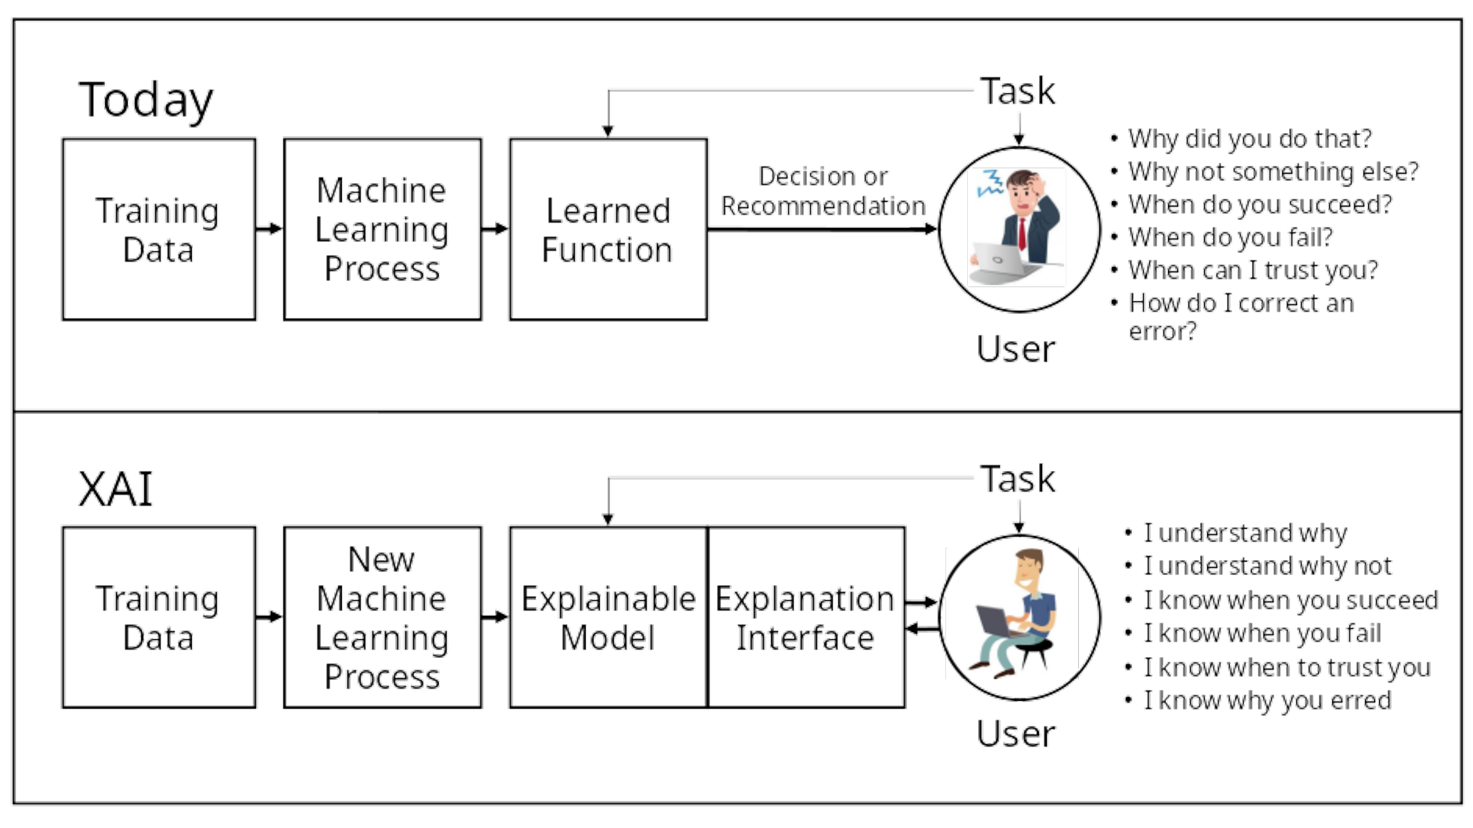
\includegraphics[width=\linewidth]{figures/xai-concept.pdf}
    \end{center}
\end{frame}

%===============================================================================
\section{Background}
%===============================================================================

\subsection{Overview on XAI}

\begin{frame}[allowframebreaks]{Explain What?}
    \begin{block}{Most efforts are devoted to \textbf{supervised} ML, and in particular:}
        \begin{itemize}
            \item specific sorts of \alert{tasks}, e.g. classification and regression
            
            \item specific sorts of \alert{data}, e.g. images, text, or tables 
            
            \item specific sorts of \alert{predictors}, e.g. neural networks, SVM
            %
            \begin{itemize}
                \item[ie] essentially, functions of the form $f: \mathcal{X} \subseteq \mathbb{R}^n \rightarrow \mathcal{Y} \subseteq \mathbb{R}^m$
            \end{itemize}
        \end{itemize}
    \end{block}
    
    \framebreak

    Interpretability--Predictivity trade-off:
    %
    \begin{figure}
        \centering
        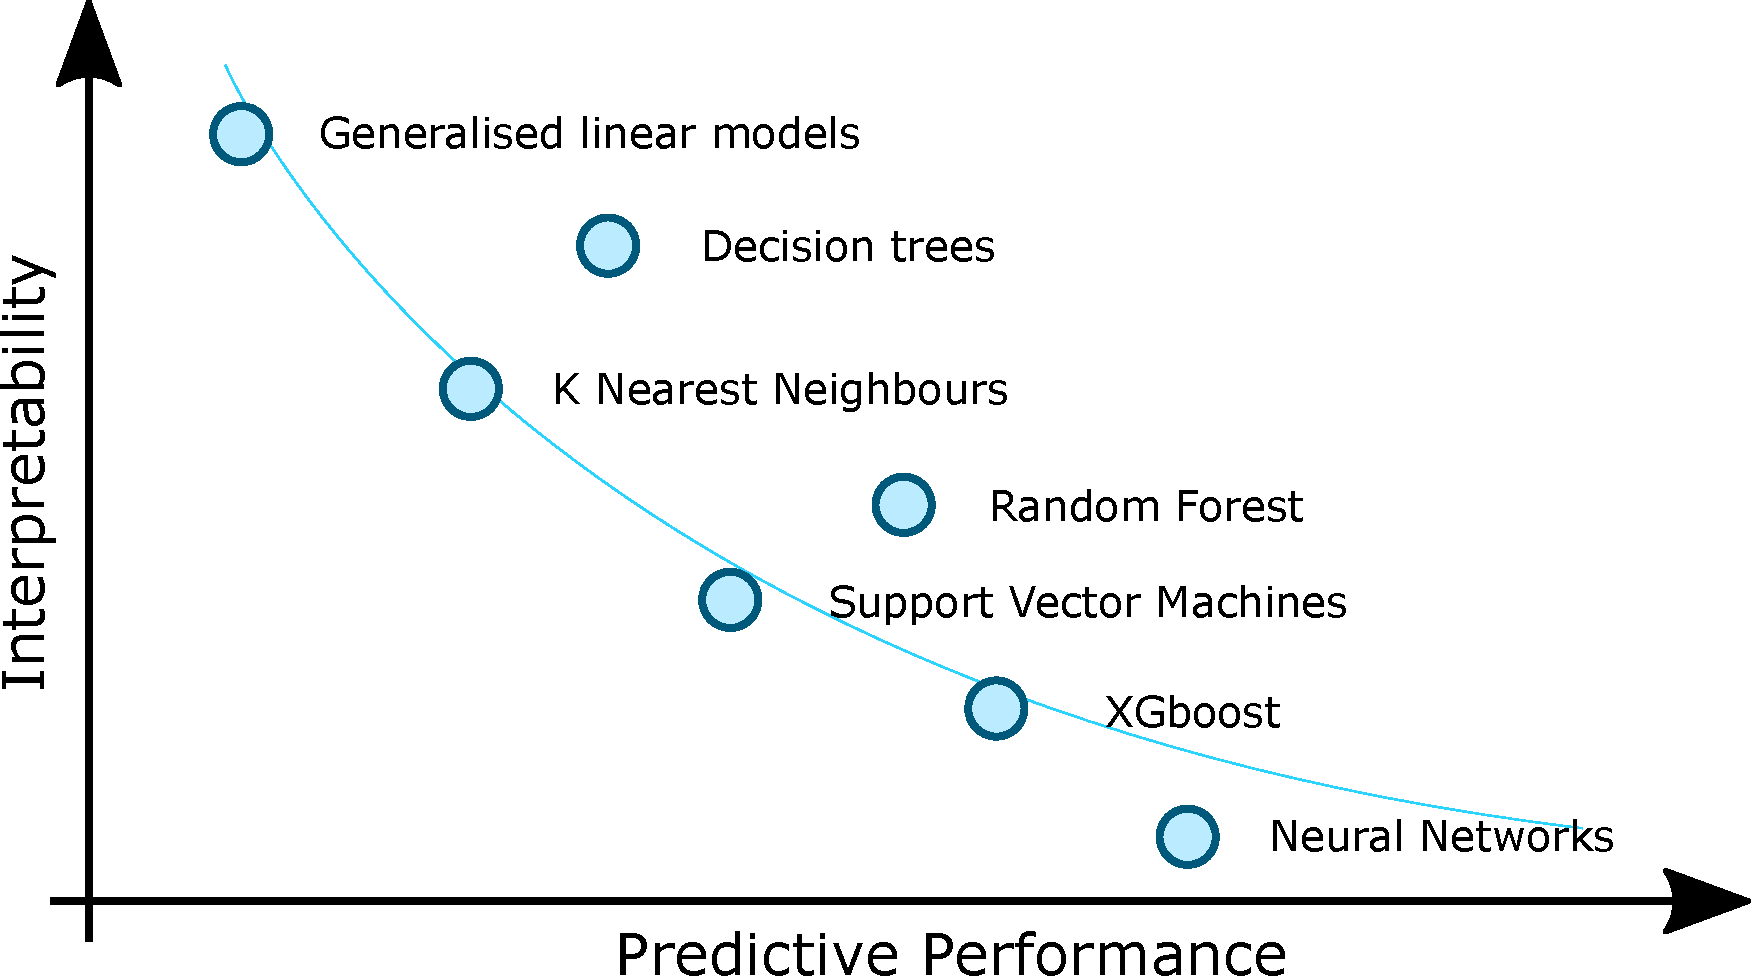
\includegraphics[width=.7\linewidth]{figures/interpretability-performance-tradeoff.pdf}
    \end{figure}

    \framebreak

    \begin{alertblock}{Conventionally\ldots}
        \begin{itemize}
            \item \ldots (generalised) linear models, or decision trees/rules are \alert{considered} interpretable
            \item \ldots other kinds of predictors are considered \alert{poorly} interpretable
            %
            \begin{itemize}
                \item hence needing \alert{explanations}
            \end{itemize}
        \end{itemize}
    \end{alertblock}
    
\end{frame}

\begin{frame}[allowframebreaks]{Global vs. Local Explanations}
    \begin{block}{Global Explanation}
        \begin{itemize}
            \item How does a predictor produces its outcomes in general?
            %
            \begin{itemize}
                \item[eg] how does a neural network classify animals?
            \end{itemize}
        \end{itemize}
    \end{block}

    \begin{block}{Local Explanation}
        \begin{itemize}
            \item How did a predictor produce a particular outcome?
            %
            \begin{itemize}
                \item[eg] why did the neural network classify a cat?
            \end{itemize}
        \end{itemize}
    \end{block}

    \framebreak

    \begin{alertblock}{About the global/local dichotomy}
        \begin{itemize}
            \item firstly introduced in \cite{Ribeiro0G16}
            \item along with \lime{}, i.e. one of the most successful XAI techniques
        \end{itemize}
    \end{alertblock}

    \framebreak

    \begin{figure}
        \centering
        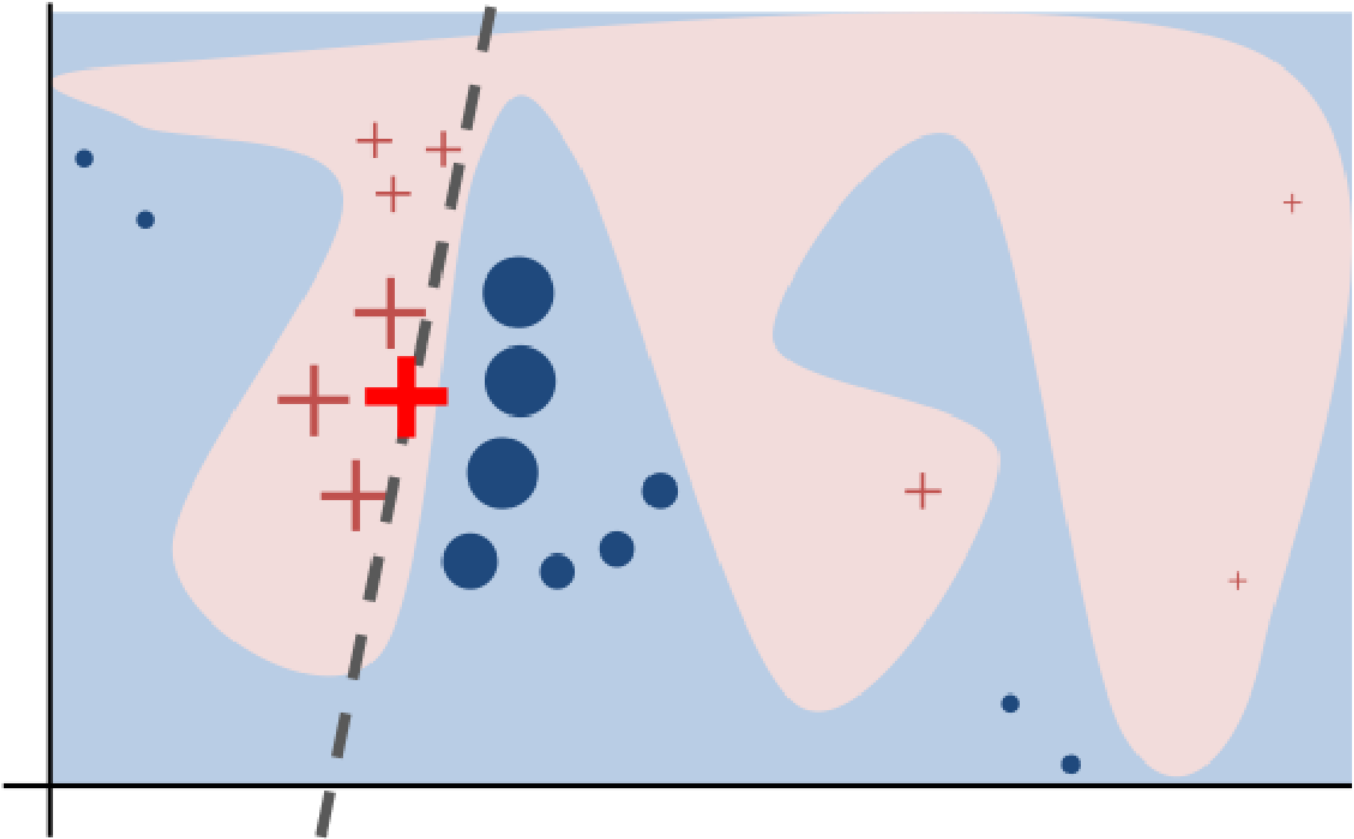
\includegraphics[width=.6\linewidth]{figures/lime.png}
        \caption{(from \cite{Ribeiro0G16}) 
Toy example to present intuition for \lime{}.
The black-box model’s complex decision function $f$ (unknown to \lime{}) is represented by the blue/pink background, which cannot be approximated well by a linear model.
The bold red cross is the instance being explained.
\lime{} samples instances, gets predictions using $f$, and weighs them by the proximity to the instance being explained (represented here by size).
The dashed line is the learned explanation that is locally (but not globally) faithful.
}
    \end{figure}
\end{frame}

\begin{frame}[allowframebreaks]{Overview on XAI approaches}
    Four major approaches, according to \cite{guidotti2018survey}:
    %
    \begin{center}
        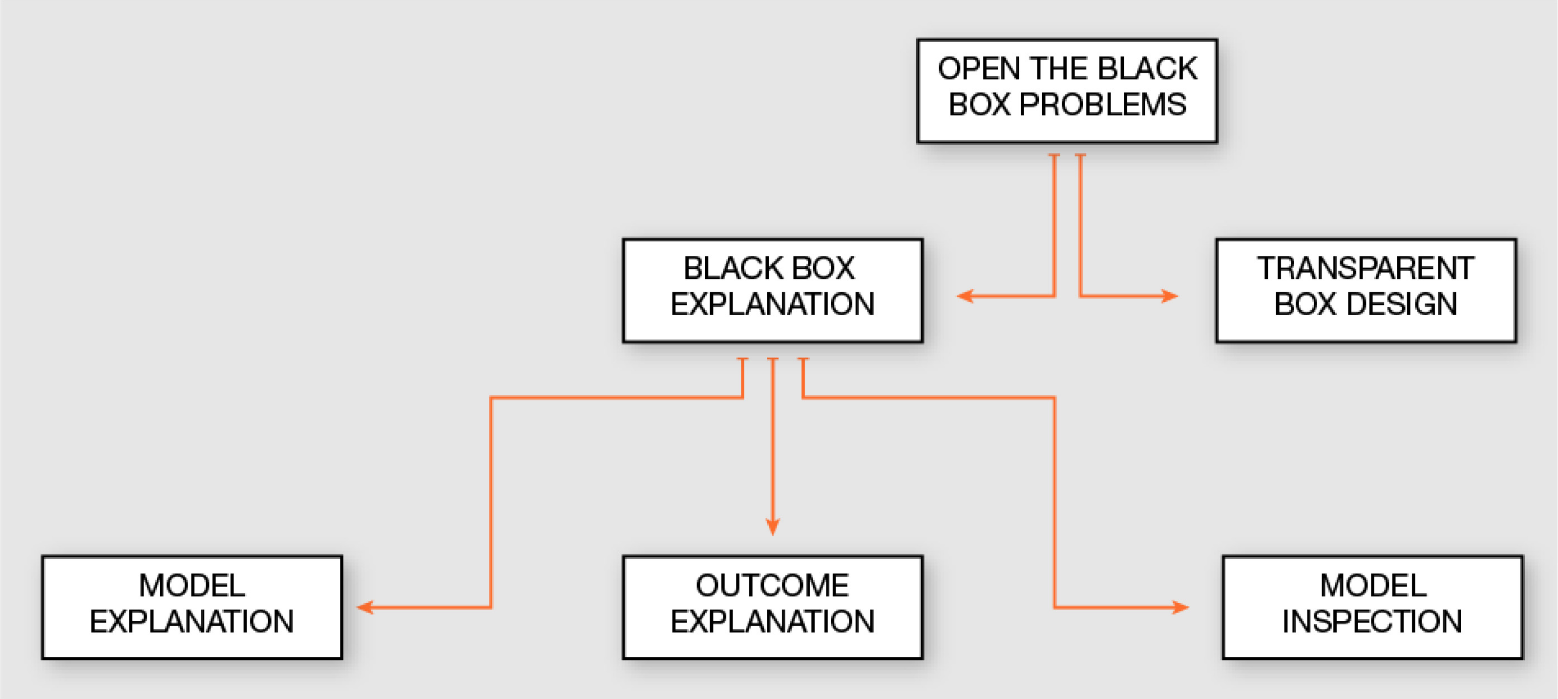
\includegraphics[width=.8\linewidth]{figures/open-bb.png}
    \end{center}

    \begin{block}{About notation}
        \begin{itemize}
            \item ``model'' $\approx$ ``predictor''
        \end{itemize}
    \end{block}
    
    \framebreak

    \begin{block}{Model Explanation ($\approx$ global explanation)}
        \begin{description}
            \item[explanation] $\approx$ interpretable predictor trained to mimic the one to be explained 
            %
            \begin{itemize}
                \item w.r.t. the entire input space
                %
                \begin{itemize}
                    \item[eg] surrogate models (e.g. decision trees)
                \end{itemize}
            \end{itemize}
        \end{description}
    \end{block}
    %
    \begin{center}
        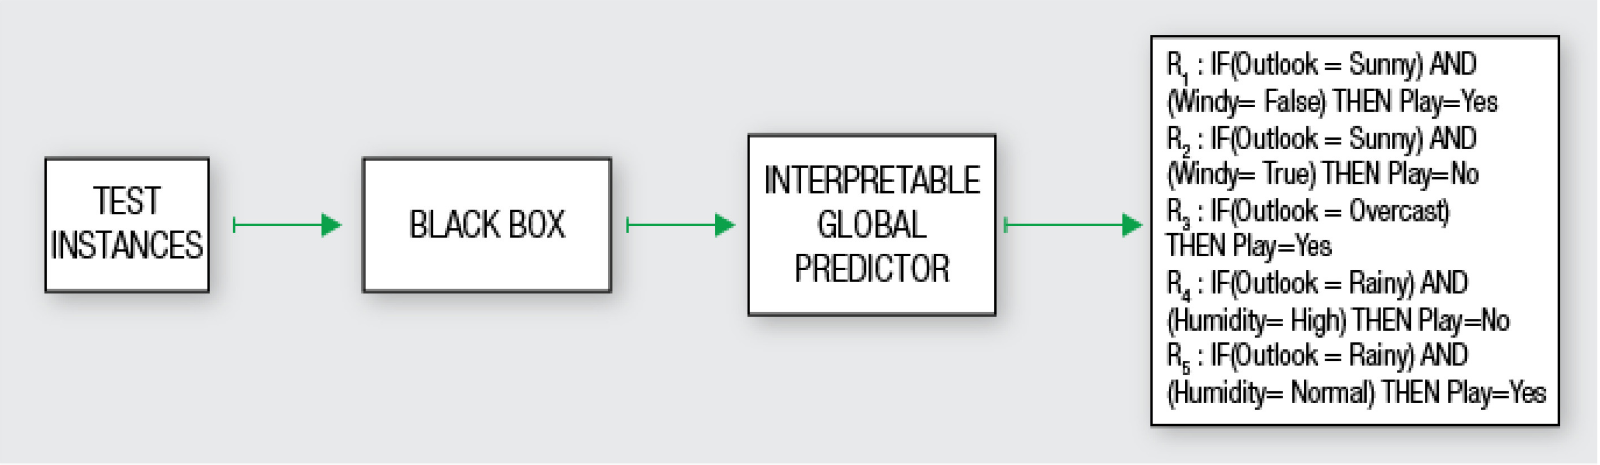
\includegraphics[width=.8\linewidth]{figures/model-explanation.png}
    \end{center}

    \framebreak

    \begin{block}{Outcome Explanation ($\approx$ local explanation)}
        \begin{description}
            \item[explanation] $\approx$ interpretable predictor trained to mimic the one to be explained
            %
            \begin{itemize}
                \item w.r.t. a small portion of the input space
                %
                \begin{itemize}
                    \item[eg] saliency maps (e.g. \lime{}\ccite{Ribeiro0G16}, SHAP\ccite{LundbergL2017})
                \end{itemize}
            \end{itemize}
        \end{description}
    \end{block}
    %
    \begin{center}
        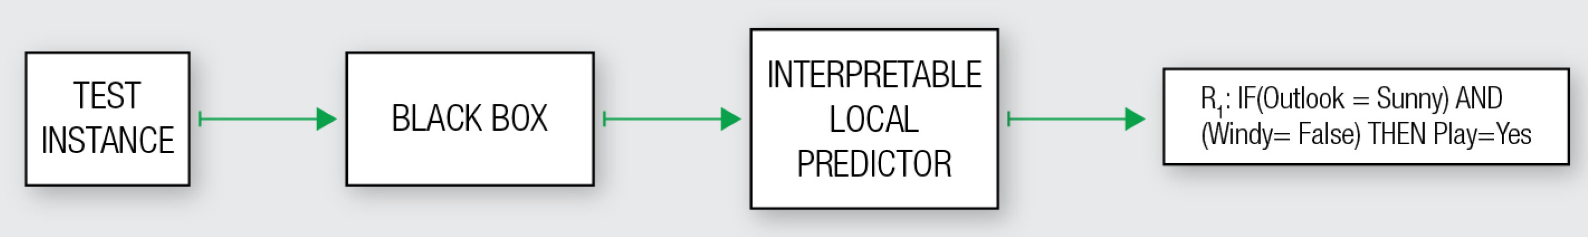
\includegraphics[width=.8\linewidth]{figures/outcome-explanation.png}
    \end{center}

    \framebreak

    \begin{block}{Model Inspection}
        \begin{description}
            \item[explanation] $\approx$ representation summarising the behaviour of the predictor to be explained 
            %
            \begin{itemize}
                \item w.r.t. a given portion of the input space (or, possibly, all of it)
                %
                \begin{itemize}
                    \item[eg] feature importance, sensitivity analysis
                \end{itemize}
            \end{itemize}
        \end{description}
    \end{block}
    %
    \begin{center}
        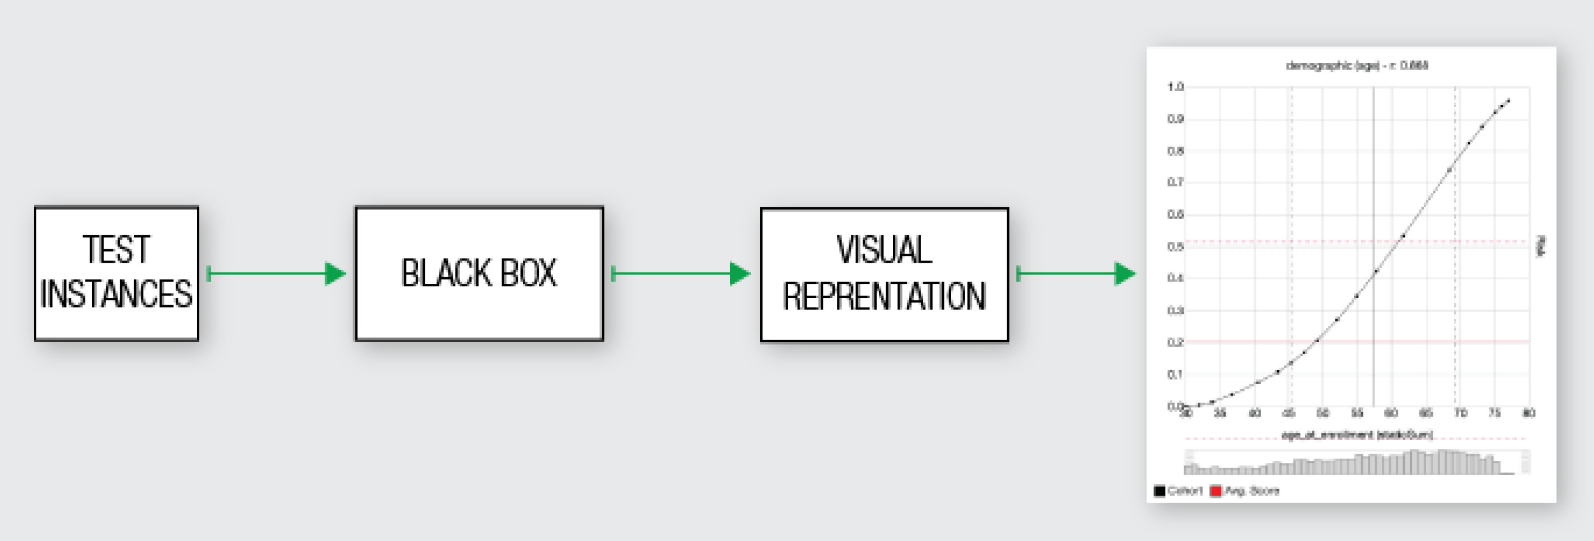
\includegraphics[width=.8\linewidth]{figures/model-inspection.png}
    \end{center}

    \framebreak

    \begin{block}{Transparent Box Design}
        \begin{itemize}
            \item just train an interpretable predictor and look at it
        \end{itemize}
    \end{block}
    %
    \begin{center}
        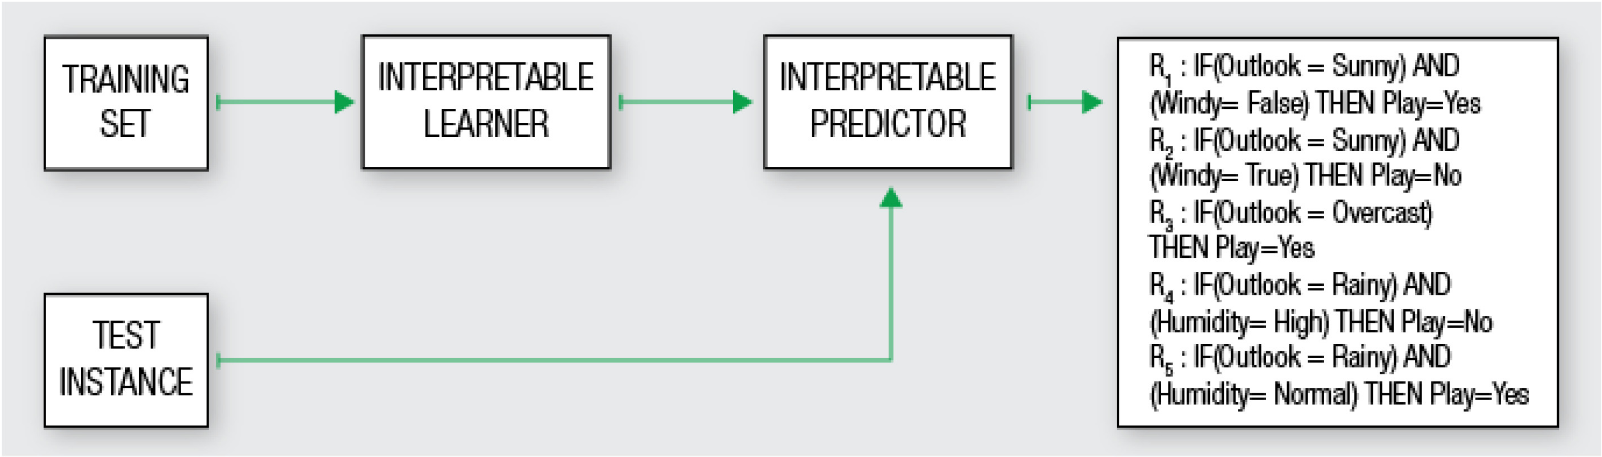
\includegraphics[width=.8\linewidth]{figures/transparent-box-design.png}
    \end{center}
\end{frame}

\subsection{Interpretation vs. Explanation}

\begin{frame}{Interpretation or Explanation?}

    The two terms are \alert{not} interchangeable
    %
    \begin{itemize}
        \item \ldots despite they are often used interchangeably
    \end{itemize}

    \vfill

    \begin{block}{Insights}
        \begin{description}
            \item[interpretation] $\approx$ binding objects with meaning
            %
            \begin{itemize}
                \item that's what the human mind does
            \end{itemize}

            \item[explanation] $\approx$ eliciting relevant aspects of objects (to ease their interpretation)
        \end{description}
    \end{block}
\end{frame}

\begin{frame}{The Role of Representations}

    \begin{center}
        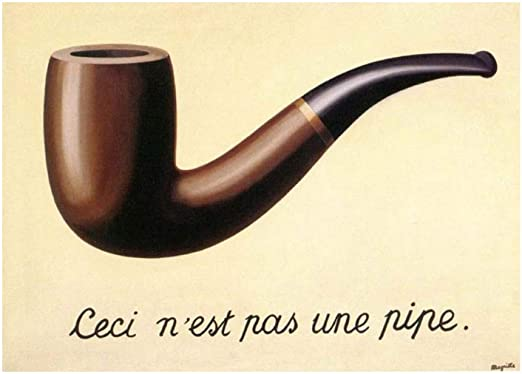
\includegraphics[width=.7\linewidth]{figures/pipe.jpg}
    \end{center}
    %
    \begin{itemize}
        \item[!] this is just a \alert{representation} of a pipe
    \end{itemize}

\end{frame}

\begin{frame}[allowframebreaks]{An abstract framework for XAI\ccite{agentbasedxai-extraamas2020}}

    \begin{center}
        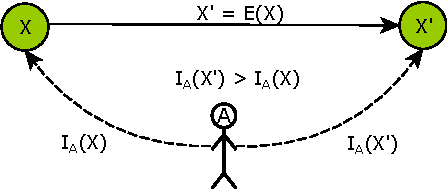
\includegraphics[width=.5\linewidth]{figures/framework.pdf}
    \end{center}
    %
    \begin{itemize}
        \item[$X$] object to be explained
        \item[$A$] observer agent
        \item[$I_A(\cdot)$] a function ``measuring'' the ``degree of interpretability'' of $X$, w.r.t. $A$
        \item[$E(\cdot)$] an \alert{explanation} function, mapping objects into (different) objects      
        \item[$X'$] the \alert{result} of the explanation, i.e. a \alert{more-interpretable} object
    \end{itemize}
    
    \begin{block}{Key points}
        \begin{itemize}
            \item interpretation is \alert{subjective}
            \item explanation is an operation transforming poorly interpretable objects into more-interpretable ones
            \item `interpretability' does not need to be measurable (only comparisons matter)
        \end{itemize}
    \end{block}

    \framebreak

    In the particular case of ML-based AI:
    %
    \begin{center}
        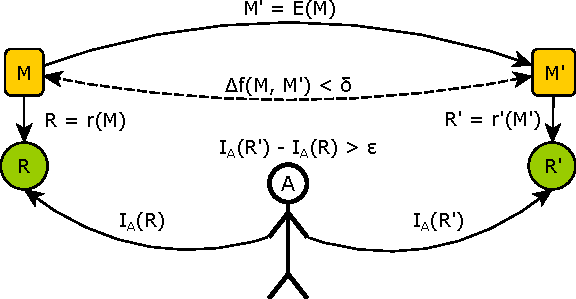
\includegraphics[width=\linewidth]{figures/global.pdf}
    \end{center}
    %
    \framebreak
    %
    \begin{itemize}
        \item we need to explain a model $M$
        %
        \begin{itemize}
            \item having a poorly interpretable \alert{representation} $R$ (w.r.t. $A$)
        \end{itemize}

        \item explanation produces another model $M'$
        %
        \begin{itemize}
            \item having an interpretable \alert{representation} $R'$ (w.r.t. $A$)
        \end{itemize}

        \item performance difference among $M$ and $M'$ (i.e. $\Delta f(M, M')$) must be small ($< \delta$)
        %
        \begin{itemize}
            \item or, dually, $M'$ must have an high \alert{fidelity} w.r.t. $M$
        \end{itemize}
    \end{itemize}

    \begin{block}{Key points}
        \begin{itemize}
            \item explanation $\approx$ search of a \alert{surrogate} interpretable model
            \item \alert{representation} is important as much as explanation
            \item explanation must maximise \alert{fidelity}
        \end{itemize}
    \end{block}

\end{frame}

\subsection{Explanations via Symbolic Knowledge Extraction}

\begin{frame}[allowframebreaks]{Overview}
    \begin{columns}
        \begin{column}{0.19\linewidth}
            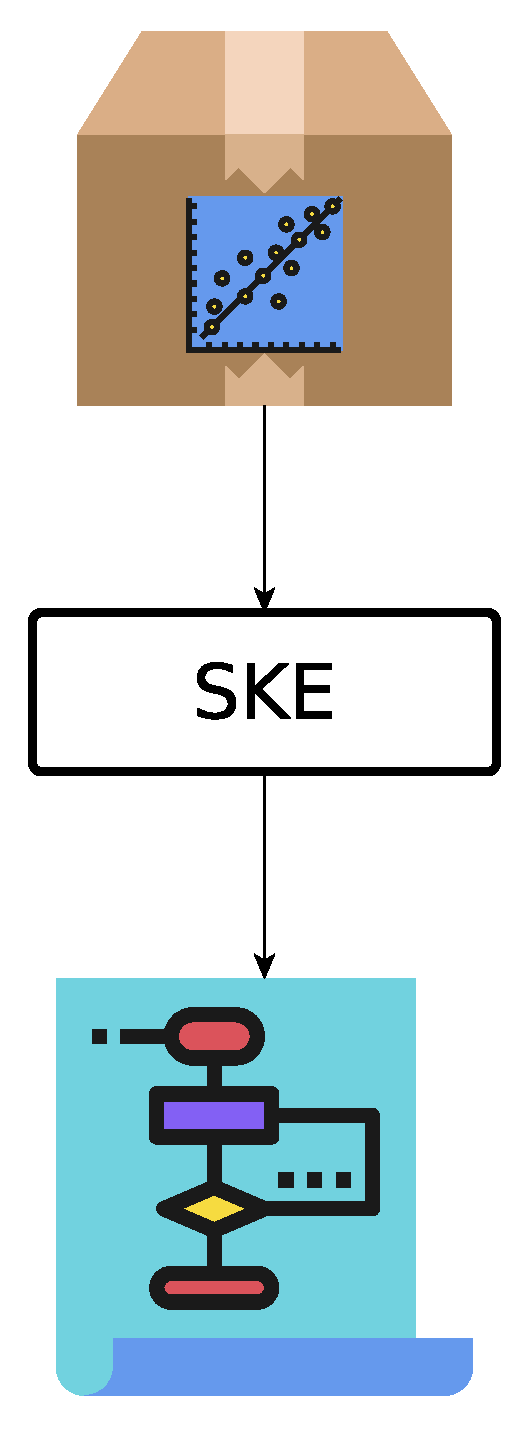
\includegraphics[width=\linewidth]{figures/ske.pdf}
        \end{column}
        \hfill
        \begin{column}{0.8\linewidth}
            \begin{block}{Insight}
                \begin{itemize}
                    \item search of a \alert{surrogate} interpretable model\ldots
                    \medskip
                    \item \ldots consisting of \alert{symbolic knowledge}
                \end{itemize}
            \end{block}
        \end{column}
    \end{columns}

    \framebreak

    \begin{block}{Definition: Symbolic Knowledge Extraction (SKE)}\centering\itshape
        Any \emph{algorithmic} procedure accepting \emph{trained} sub-symbolic predictors as input and producing \emph{symbolic} knowledge as output, in such a way that the extracted knowledge reflects the behaviour of the predictor with high \emph{fidelity}.
    \end{block}

    \framebreak

    Example:
    %
    \begin{columns}
        \begin{column}{.43\linewidth}
            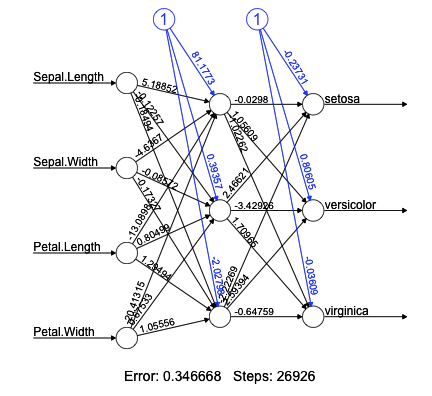
\includegraphics[width=\linewidth]{figures/nn-iris.png}
        \end{column}
        $\rightarrow$
        \begin{column}{.53\linewidth}\small
            \[ 
                \begin{array}{l}
                    \variable{Class} = \functor{setosa} \leftarrow \variable{PetalWidth} \leq 1.0 \fullstop
                    \\
                    \\
                    \variable{Class} = \functor{versicolor} \leftarrow \variable{PetalLength} > 4.9 \\ 
                        \qquad  \wedge\ \variable{SepalWidth} \in [2.9,\ 3.2] \fullstop
                    \\
                    \variable{Class} = \functor{versicolor} \leftarrow  \variable{PetalWidth} > 1.6 \fullstop
                    \\
                    \\
                    \variable{Class} = \functor{virginica} \leftarrow \variable{SepalWidth} \leq 2.9 \fullstop
                    \\
                    \\
                    \variable{Class} = \functor{virginica} \leftarrow \\ 
                        \qquad \variable{SepalLength} \in [5.4,\ 6.3] \fullstop
                    \\
                    \variable{Class} = \functor{virginica} \leftarrow \\ 
                        \qquad \variable{PetalWidth} \in [1.0,\ 1.6] \fullstop
                \end{array}    
            \]
        \end{column}
    \end{columns}
\end{frame}

\begin{frame}[allowframebreaks]{What does `symbolic' actually mean?}
    According to \cite{Gelder90}, \alert{symbolic} representations of knowledge
    %
    \begin{itemize}
        \item involves a \alert{set of symbols},
        \item which can be combined (e.g., concatenated) in (possibly) \alert{infinitely many} ways, 
        \item following precise \alert{syntactical} rules, and
        \item where both elementary symbols and any admissible combination of them can be assigned with \alert{meaning}
        %
        \begin{itemize}
            \item[ie] \alert{each} symbol can be mapped into some entity from the domain at hand.
        \end{itemize}
    \end{itemize}
    
    \begin{exampleblock}{Notable example}
        \begin{itemize}
            \item formal logic
        \end{itemize}
    \end{exampleblock}

    \framebreak

    \begin{alertblock}{Opposite notion: \textbf{distributed} representations}
        \begin{itemize}
            \item where symbols \alert{alone} have no meaning
            \item unless it is considered along with its \alert{neighbourhood}
            %
            \begin{itemize}
                \item[ie] any other symbol which is \alert{close} (according to some notion of closeness)
            \end{itemize}
        \end{itemize}
    \end{alertblock}
\end{frame}

\begin{frame}[allowframebreaks]{Plenty of SKE methods from the literature}
    % !TeX root = ../ise-lab-ske.tex

\newcommand{\myhead}{
	\textbf{\#} & \textbf{Method} & \textbf{Translucency} & \textbf{Task} & \textbf{Input} & \textbf{Expressiveness} & \textbf{Shape} 
    \\\hline\hline
}

\newcounter{SkeMethod}
\setcounter{SkeMethod}{1}
\newcommand{\newSkeMethodIndex}{\theSkeMethod\stepcounter{SkeMethod}}

\begin{scriptsize}
\begin{longtable}{c|p{3cm}|c|c|c|c|c}
    % first header
    \caption{
        Summary of the knowledge-extraction algorithms.
        %
        Symbol $*$ means that the related dimension of the algorithm is not bounded.
        %
        Symbol $\dagger$ means that the output is a power law.
    }
    \label{tab:ske-taxonomy}
    \\
    \myhead
    %
    \newSkeMethodIndex & \cite{breiman1984classification} & P & C+R & C+D & P & DT 
    \\\hdashline
    \newSkeMethodIndex & \cite{Quinlan86ID3} & P & C & D & P & DT 
    \\\hdashline
    \newSkeMethodIndex & \cite{SaitoN88} & P & C & D & P & L 
    \\\hdashline
    \newSkeMethodIndex & \cite{ClarkN89} & P & C & C+D & P & L 
    \\\hline
    \newSkeMethodIndex & \cite{Masuoka1990} & D (NN) & C & C & F & L 
    \\\hdashline
    \newSkeMethodIndex & \cite{Hayashi90} & D (NN) & C & B & F & L 
    \\\hdashline
    \newSkeMethodIndex & \cite{TowellS91} & D (NN) & C & D & MN & L 
    \\\hdashline
    \newSkeMethodIndex & \cite{Berenji91} & D (NN) & C & C & F & L 
    \\\hdashline
    \newSkeMethodIndex & \cite{BrunkP91} & P & C & C+D & P & L 
    \\\hdashline
    \newSkeMethodIndex & \cite{murphy1991id2} & P & C & D & MN & DT 
    \\\hdashline
    \newSkeMethodIndex & \cite{HorikawaFU92} & D (NN) & C & C & F & L 
    \\\hdashline
    \newSkeMethodIndex & \cite{TrespHA92} & D (NN) & R & C & P & L 
    \\\hdashline
    \newSkeMethodIndex & \cite{towell1993extracting} & D (NN) & C & D & P & L 
    \\\hdashline
    \newSkeMethodIndex & \cite{Thrun1993ExtractingPC} & D (NN) & C & C & P+MN & L 
    \\\hdashline
    \newSkeMethodIndex & \cite{Cohen93} & P & C & C+D & P & L 
    \\\hdashline
    \newSkeMethodIndex & \cite{quinlan1993c4} & P & C & C+D & P & DT 
    \\\hdashline
    \newSkeMethodIndex & \cite{Fu94} & D (NN) & C & D & P & L 
    \\\hdashline
    \newSkeMethodIndex & \cite{halgamuge1994neural} & D (NN) & C & C & F & L 
    \\\hdashline
    \newSkeMethodIndex & \cite{MITRA1994285} & D (NN) & C & C+D & F & L 
    \\\hdashline
    \newSkeMethodIndex & \cite{craven1994using} & P & C & B & P+MN & L 
    \\\hdashline
    \newSkeMethodIndex & \cite{FurnkranzW94} & P & C & D & P & L 
    \\\hdashline
    \newSkeMethodIndex & \cite{sestito94automated} & P & C & C & P & L 
    \\\hline
    \newSkeMethodIndex & \cite{Andrews95rulex} & D (NN) & C & C+D & P & L 
    \\\hdashline
    \newSkeMethodIndex & \cite{Matthews95fuzzy} & D (NN) & C & B & F & L 
    \\\hdashline
    \newSkeMethodIndex & \cite{Cohen95} & P & C & C+D & P & L 
    \\\hdashline
    \newSkeMethodIndex & \cite{PopTHSD95} & P & C & B & P & L 
    \\\hdashline
    \newSkeMethodIndex & \cite{SetionoL96} & D (NN) & C & B & P & L 
    \\\hdashline
    \newSkeMethodIndex & \cite{tickle1996dedec} & P & C & B & P & L 
    \\\hdashline
    \newSkeMethodIndex & \cite{YuanZ96} & P & C & D & F & L 
    \\\hdashline
    \newSkeMethodIndex & \cite{craven1996extracting} & P & C & B & P+MN & DT 
    \\\hdashline
    \newSkeMethodIndex & \cite{HongL96} & P & C & C & F & L 
    \\\hdashline
    \newSkeMethodIndex & \cite{Setiono97NeuroLinear} & D (NN3) & C & C+D & O & L 
    \\\hdashline
    \newSkeMethodIndex & \cite{Setiono97a} & D (NN) & C & D & P & L 
    \\\hdashline
    \newSkeMethodIndex & \cite{NauckK97} & D (NN) & C & D & F & L 
    \\\hdashline
    \newSkeMethodIndex & \cite{SaitoN97} & D (NN) & R & C & $\dagger$ & $\dagger$ 
    \\\hdashline
    \newSkeMethodIndex & \cite{BenitezCR97} & D (NN) & C+R & C & F & L 
    \\\hdashline
    \newSkeMethodIndex & \cite{IshibuchiNM97} & P & C & C & F & L 
    \\\hdashline
    \newSkeMethodIndex & \cite{TahaG99} & D (NN) & C & C & P & L 
    \\\hdashline
    \newSkeMethodIndex & \cite{TahaG99} & D (NN) & C & C & P & L 
    \\\hdashline
    \newSkeMethodIndex & \cite{Krishnan99combo} & D (NN) & C & B & P & L 
    \\\hdashline
    \newSkeMethodIndex & \cite{NauckK99} & D (NN) & R & D & F & L 
    \\\hdashline
    \newSkeMethodIndex & \cite{TahaG99} & P & C & B & P & L 
    \\\hdashline
    \newSkeMethodIndex & \cite{KrishnanSB99} & P & C & C & P & DT 
    \\\hdashline
    \newSkeMethodIndex & \cite{schmitz1999NN} & P & C+R & C+D & P & DT 
    \\\hdashline
    \newSkeMethodIndex & \cite{HongC99} & P & C & C & F & L 
    \\\hline
    \newSkeMethodIndex & \cite{Setiono00} & D (NN) & C & B & MN & L 
    \\\hdashline
    \newSkeMethodIndex & \cite{Tsukimoto00} & D (NN) & C & C+D & P & L 
    \\\hdashline
    \newSkeMethodIndex & \cite{Kim2000} & D (NN4) & C & C+D & P & DT 
    \\\hdashline
    \newSkeMethodIndex & \cite{SetionoL00} & D (NN) & R & C+D & P+MN+O & DT 
    \\\hdashline
    \newSkeMethodIndex & \cite{ZhouCC00} & P & C & C+D & P & L 
    \\\hdashline
    \newSkeMethodIndex & \cite{HongC00a} & P & C & C & F & L 
    \\\hdashline
    \newSkeMethodIndex & \cite{sato2001rule} & D (NN3) & R & C+D & P & DT 
    \\\hdashline
    \newSkeMethodIndex & \cite{parpinelli2001ant} & P & C & C+D & P & L 
    \\\hdashline
    \newSkeMethodIndex & \cite{CastilloGP01} & P & C+R & C+D & F & L 
    \\\hdashline
    \newSkeMethodIndex & \cite{saito2002extracting} & D (NN) & R & C+D & P & L 
    \\\hdashline
    \newSkeMethodIndex & \cite{setiono2002extraction} & D (NN3) & R & C+D & P & L 
    \\\hdashline
    \newSkeMethodIndex & \cite{liu2002density} & P & C & C+D & P & L 
    \\\hdashline
    \newSkeMethodIndex & \cite{Boz02} & P & C & C+D & P & DT 
    \\\hdashline
    \newSkeMethodIndex & \cite{Markowska-KaczmarT03} & P & C & C+D & F & L 
    \\\hdashline
    \newSkeMethodIndex & \cite{ZhouJC03} & P & C & C+D & P & L 
    \\\hdashline
    \newSkeMethodIndex & \cite{SetionoT04} & D (NN3) & R & C+D & P & L 
    \\\hdashline
    \newSkeMethodIndex & \cite{Fu2004} & D (SVM) & C & C+D & P & L 
    \\\hdashline
    \newSkeMethodIndex & \cite{Markowska-KaczmarC04} & P & C & C+D & P & L 
    \\\hdashline
    \newSkeMethodIndex & \cite{RabunalDPPR04} & P & C & C+D & P & L 
    \\\hdashline
    \newSkeMethodIndex & \cite{Chen2004LEARNINGAA} & P & C & C & P & L 
    \\\hdashline
    \newSkeMethodIndex & \cite{LiuAM04} & P & C & C+D & P & L 
    \\\hdashline
    \newSkeMethodIndex & \cite{Browne2004} & P & C & C+D & P+MN & DT 
    \\\hline
    \newSkeMethodIndex & \cite{ZhangSJC05} & D (SVM) & C & C & P & L 
    \\\hdashline
    \newSkeMethodIndex & \cite{barakat2005eclectic} & D (SVM) & C+R & * & * & * 
    \\\hdashline
    \newSkeMethodIndex & \cite{FungSR05} & D (SVM+LC) & C & C & P & L 
    \\\hdashline
    \newSkeMethodIndex & \cite{ChavesVT05} & D (SVM) & C & C & F & L 
    \\\hdashline
    \newSkeMethodIndex & \cite{Torres2005} & P & C & C+D & P+MN & DT 
    \\\hdashline
    \newSkeMethodIndex & \cite{EtchellsL06} & P & C & C+D & P & L 
    \\\hdashline
    \newSkeMethodIndex & \cite{He2006} & P & C & C+D & P & DT 
    \\\hdashline
    \newSkeMethodIndex & \cite{huysmans2006iter} & P & R & C & P & L 
    \\\hdashline
    \newSkeMethodIndex & \cite{BaderHM07} & D (NN) & C & B & P & L 
    \\\hdashline
    \newSkeMethodIndex & \cite{SchetininFPCKEBH07} & D (DTE) & R & C & P & DT 
    \\\hdashline
    \newSkeMethodIndex & \cite{ChenLW07} & D (SVM) & C & C & P & L 
    \\\hdashline
    \newSkeMethodIndex & \cite{BarakatB07} & D (SVM) & C & C+D & P & L 
    \\\hdashline
    \newSkeMethodIndex & \cite{SaadW07} & P & C & C+D & O & L 
    \\\hdashline
    \newSkeMethodIndex & \cite{MartensBHVSB07} & P & C & C+D & P & L 
    \\\hdashline
    \newSkeMethodIndex & \cite{NunezAC08} & D (SVM) & C & C & P+O & L 
    \\\hdashline
    \newSkeMethodIndex & \cite{SetionoBM08} & P & C & C+D & P+O & L
    \\\hdashline
    \newSkeMethodIndex & \cite{OdajimaHTS08} & P & C & D & P & L 
    \\\hdashline
    \newSkeMethodIndex & \cite{grex-icdm2008} & P & C+R & C+D & F & DT 
    \\\hdashline
    \newSkeMethodIndex & \cite{Bader09} & D (NN) & C & B & P & L 
    \\\hdashline
    \newSkeMethodIndex & \cite{MartensBG09} & D (SVM) & C & * & * & * 
    \\\hline
    \newSkeMethodIndex & \cite{LehmannBH10} & P & C & B & P & L 
    \\\hdashline
    \newSkeMethodIndex & \cite{AugastaK12} & P & C & C+D & P & L 
    \\\hdashline
    \newSkeMethodIndex & \cite{sethi2012kdruleex} & P & C & C+D & P & TA 
    \\\hline
    \newSkeMethodIndex & \cite{ZilkeMJ16} & D (NN) & R & C+D & P & DT 
    \\\hdashline
    \newSkeMethodIndex & \cite{ChanC17} & D (NN) & R & C & P & L 
    \\\hdashline
    \newSkeMethodIndex & \cite{YedjourB18} & P & C & B & P & L 
    \\\hdashline
    \newSkeMethodIndex & \cite{CHAN2020329} & D (NN) & R & C & P & L 
    \\\hline
    \newSkeMethodIndex & \cite{WangWWYWJ20} & D (DTE) & C & C & P & L 
    \\\hdashline
    \newSkeMethodIndex & \cite{gridex-extraamas2021} & P & R & C & P & L 
\end{longtable}
\end{scriptsize}

% Regex per togliere gli acronimi (incompleta al momento)
% ([a-z]|[A-Z]|\\|[0-9]|\{|\}| |\.|\-|\+|\[|\])* &

\end{frame}

\begin{frame}[allowframebreaks]{Taxonomy of SKE methods}
    \begin{center}
        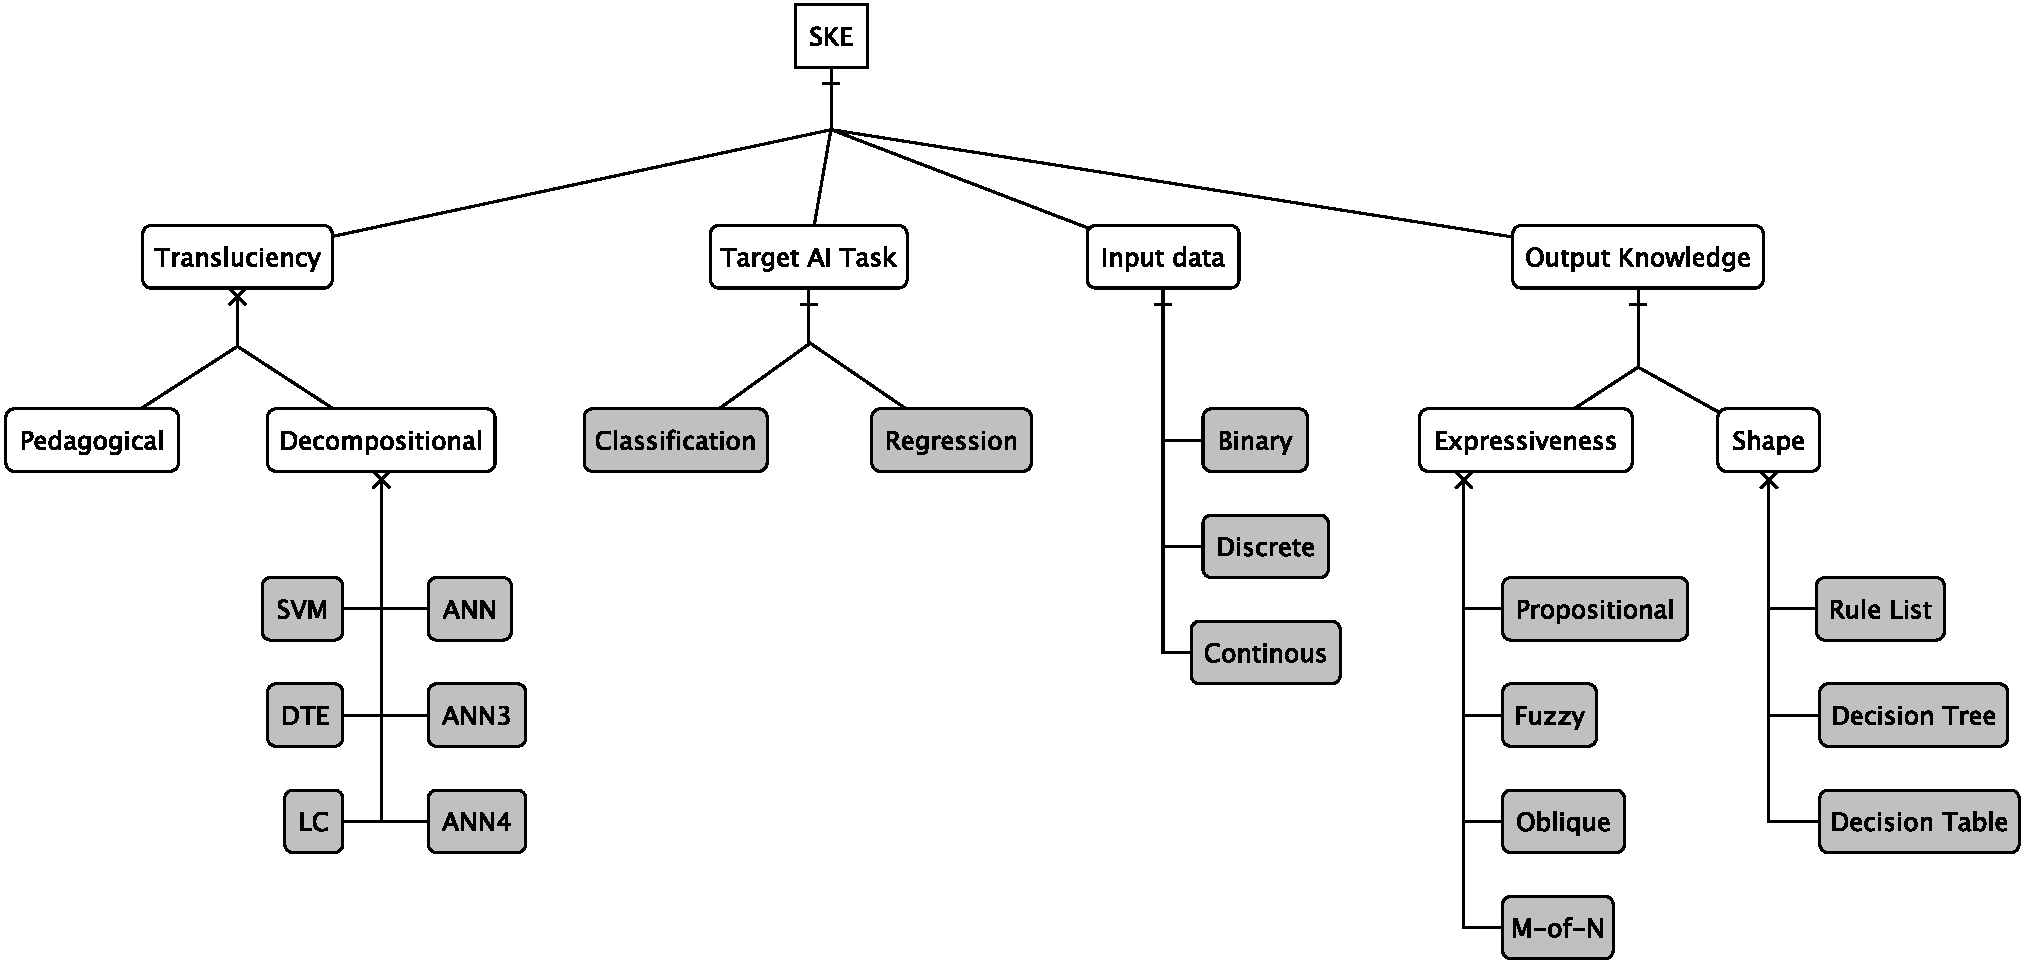
\includegraphics[width=\linewidth]{figures/ske-taxonomy.pdf}
    \end{center}
    
    \framebreak

    \begin{description}
        \item[target AI task] for the predictor undergoing extraction
        %
        \begin{description}
            \item[classification] i.e., $f: \mathcal{X} \subseteq \mathbb{R}^n \rightarrow \mathcal{Y}$ s.t. $|\mathcal{Y}| = k$
            \item[regression] i.e., $f: \mathcal{X} \subseteq \mathbb{R}^n \rightarrow \mathcal{Y} \subseteq \mathbb{R}^m$     
        \end{description} 

        \medskip

        \item[translucency] what kind of ML predictor does the SKE method support?
        %
        \begin{description}
            \item[pedagogical:] any supervised predictor
            \item[decompositional:] a particular sort of ML predictor (e.g. NN, SVM, DT)      
        \end{description} 

        \medskip

        \item[input data] supported by the predictor undergoing extraction
        %
        \begin{description}
            \item[binary:] $\mathcal{X} \equiv \{0, 1\}^n$
            \item[discrete:] $\mathcal{X} \in \{x_1, \ldots, x_n\}^n$   
            \item[continuous:] $\mathcal{X} \subseteq \mathbb{R}^n$     
        \end{description} 

        \framebreak

        \item[shape] of the extracted knowledge
        %
        \begin{description}
            \item[rule list:] i.e. ordered sequences of if-then-else rules
            \item[decision tree:] hierarchical set of if-then-else rules involving a comparison among a variable and a constant   
            \item[decision table:] 2D tables summarising decisions for each possible assignment of variables
        \end{description} 

        \framebreak

        \item[expressiveness] of the extracted knowledge
        %
        \begin{description}
            \item[propositional:] boolean statements + logic connectives
            %
            \begin{itemize}
                \item there including arithmetic comparisons among variables and constants
            \end{itemize}

            \item[fuzzy:] hierarchical set of if-then-else rules involving a comparison among a variable and a constant   
            \item[oblique:] boolean statements + logic connectives + arithmetic comparisons
            \item[M-of-N:] any of the above + statements like $m-\text{of}-\{\phi_1, \ldots, \phi_n \}$
        \end{description} 

    \end{description}
\end{frame}

\begin{frame}[allowframebreaks]{Examples of methods and their classification -- \cart}
    \begin{block}{\textbf{\cart}:\ccite{breiman1984classification} classification and regression trees}
        \begin{itemize}
            \item \textbf{translucency:} pedagogical
            \item \textbf{target AI task:} classification OR regression
            \item \textbf{input data:} binary OR discrete OR continuous
            \item \textbf{shape:} decision tree
            \item \textbf{expressiveness:} propositional
        \end{itemize}
    \end{block}

    \framebreak

    \begin{figure}
        \centering
        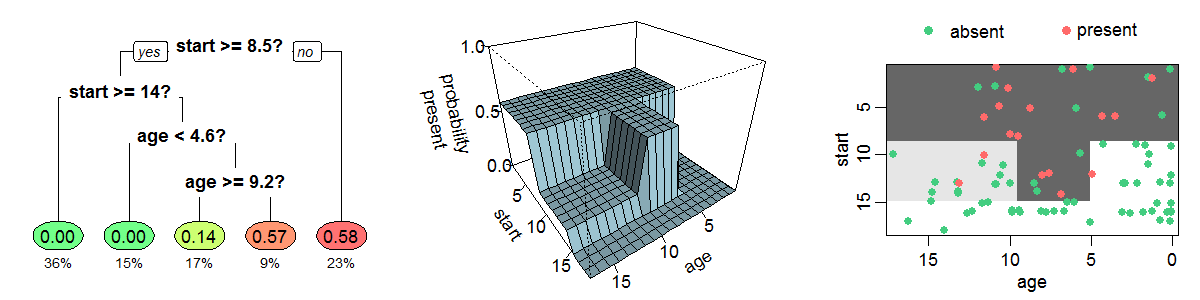
\includegraphics[width=\linewidth]{figures/dt-kyphosis.png}
        \caption{An example decision tree estimating the probability of kyphosis after spinal surgery, given the \emph{age} of the patient and the vertebra at which surgery was \emph{start}ed \cite{wiki:dt-learning}. Notice that all decision trees subtend a partition of the input space, and that those trees themselves provide intelligible representations of \emph{how} predictions are attained.}
        \label{fig:dt-example}
    \end{figure}

    \framebreak

    \begin{exampleblock}{Using \cart{} for SKE}
        \begin{enumerate}
            \item \alert{generate} a `fake' dataset by feeding the predictor undergoing SKE
            \item\label{step:dt-train} \alert{train} a decision tree on the `fake' dataset
            \item compute \alert{fidelity} and \alert{repeat} step \ref{step:dt-train} until satisfied
            \item \alert{[opt.]} rewrite the tree as a \alert{list of rules}
        \end{enumerate}
    \end{exampleblock}

\end{frame}

\begin{frame}[allowframebreaks]{Examples of methods and their classification -- \gridex}

    \begin{block}{\textbf{\gridex}:\ccite{gridex-extraamas2021} grid extractor}
        %
        \begin{itemize}
            \item \textbf{translucency:} pedagogical
            \item \textbf{target AI task:} regression
            \item \textbf{input data:} continuous
            \item \textbf{shape:} rule list
            \item \textbf{expressiveness:} propositional
        \end{itemize}
    \end{block}

    \newcommand\demodim{0.235\linewidth}

\begin{figure}\centering
	\caption{Example of \gridex{}'s hyper-cube partitioning (merging step not reported)}
	\subfloat[Surrounding\\cube]{
		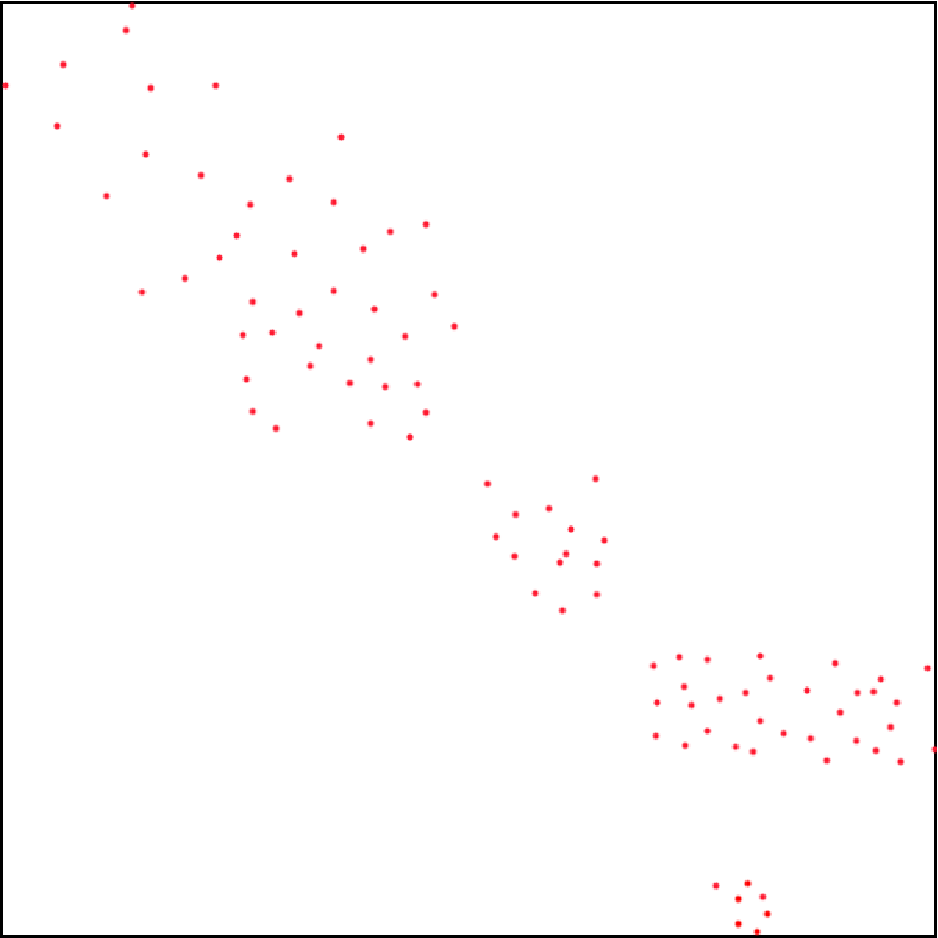
\includegraphics[width=\demodim]{figures/gridex/1.pdf}\label{fig:demo1}
	}
	\subfloat[Iteration 1 $(p_1=2)$]{
		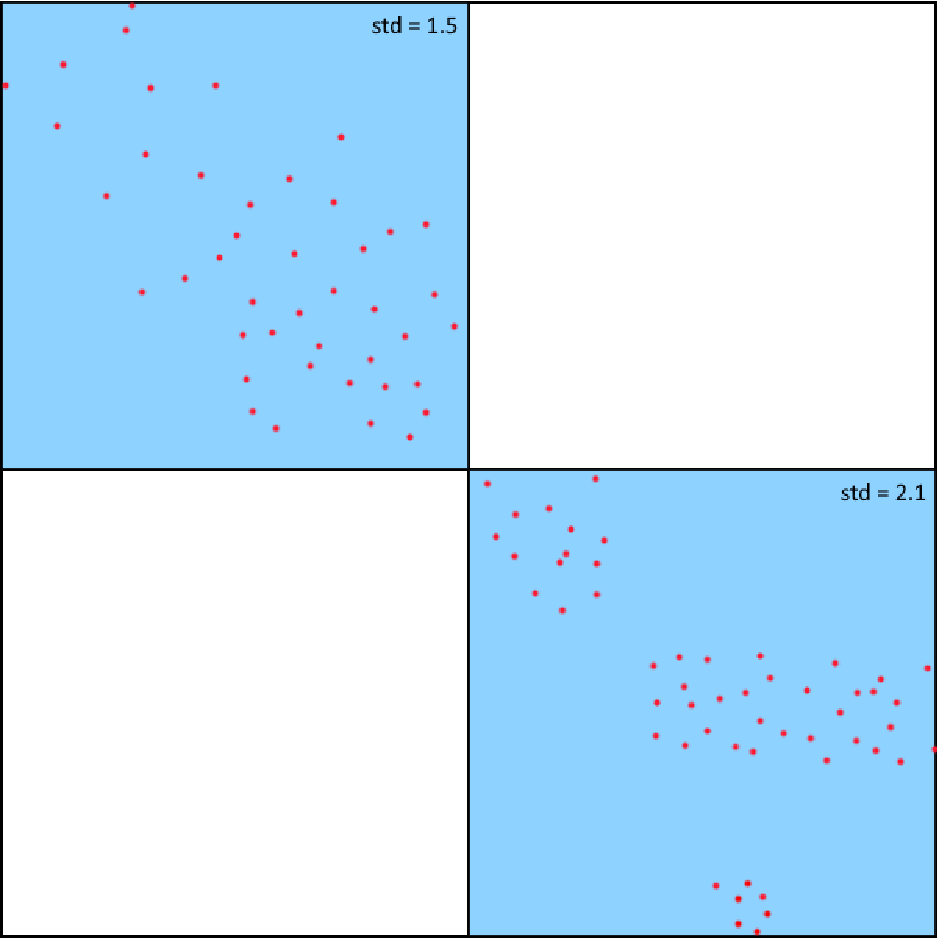
\includegraphics[width=\demodim]{figures/gridex/2.pdf}\label{fig:demo2}
	}
	\subfloat[Iteration 2 ($p_2 = 3$).]{
		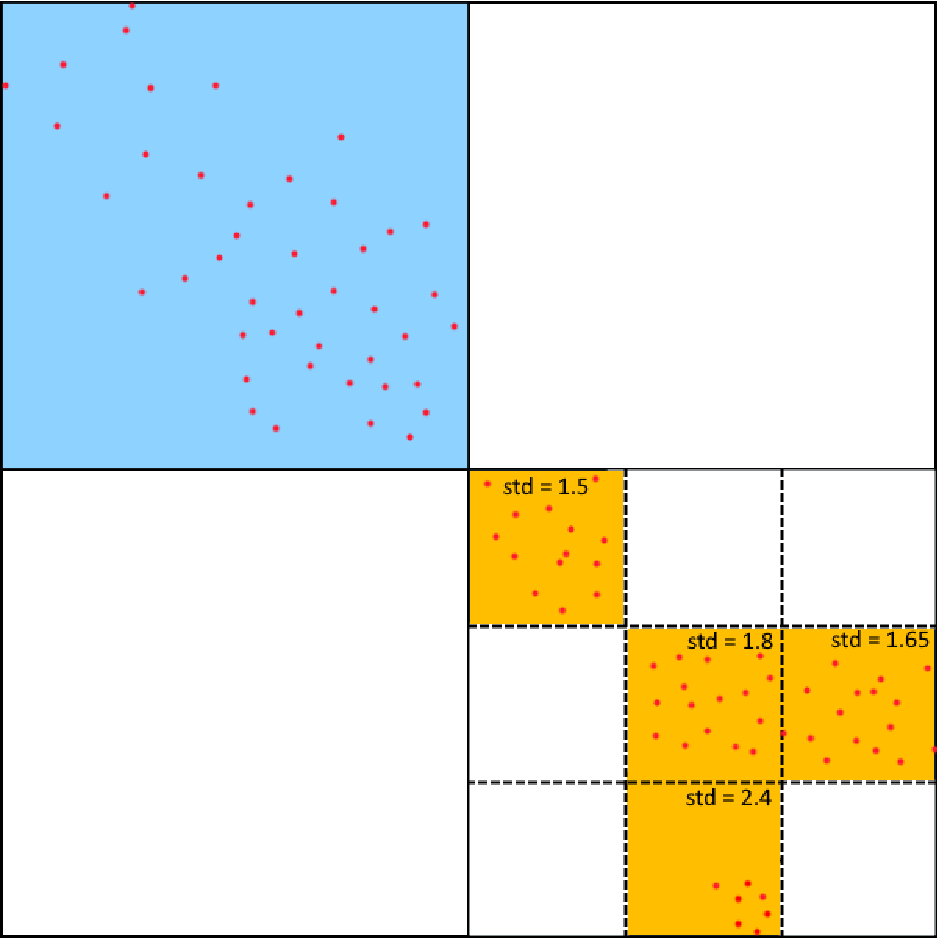
\includegraphics[width=\demodim]{figures/gridex/3.pdf}\label{fig:demo3}
	}
	\subfloat[Iteration 3 ($p_3 = 2$).]{
		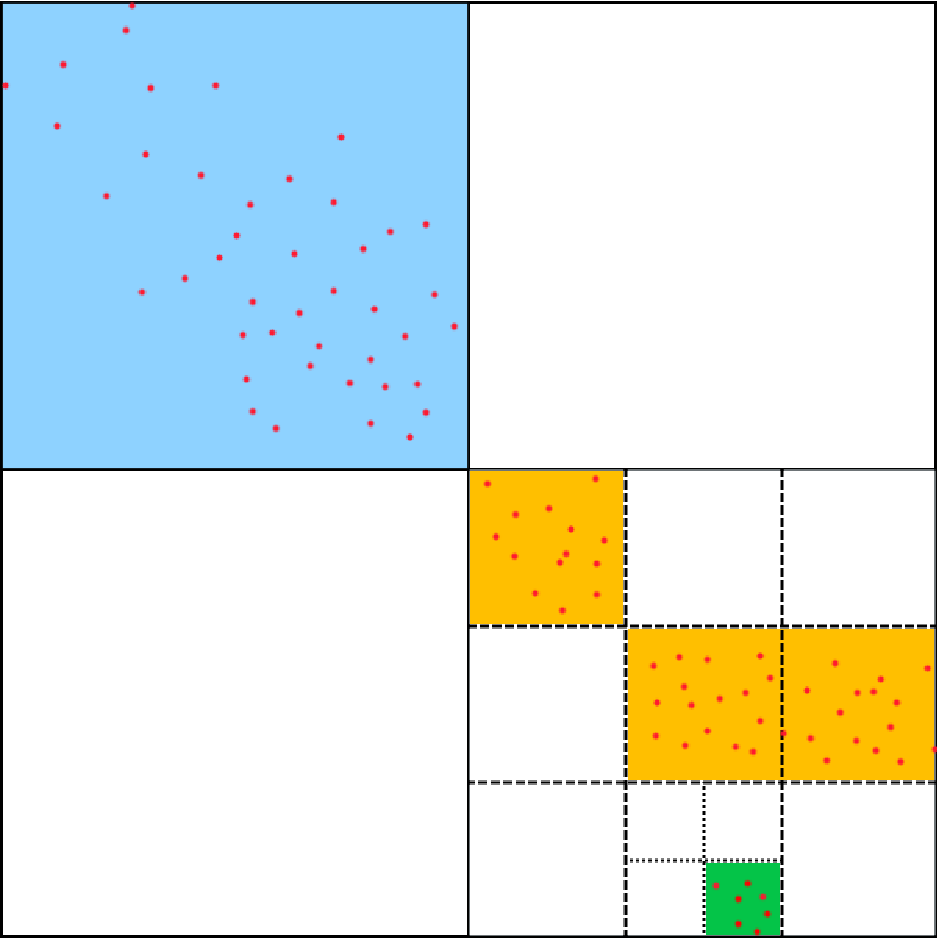
\includegraphics[width=\demodim]{figures/gridex/4.pdf}\label{fig:demo4}
	} 
\end{figure}


    \framebreak

    \begin{exampleblock}{Using \gridex{} for SKE}
        \begin{enumerate}
            \item \alert{partition} the input space into $p_1^n$ hypercubes
            %
            \begin{itemize}
                \item evenly splitting the $n$ dimensions into $p_1$ bins
            \end{itemize}
            \item \alert{partition} each non empty-region into $p_2^n$ hypercubes
            %
            \begin{itemize}
                \item evenly splitting the $n$ dimensions into $p_2$ bins
            \end{itemize}
            \item \alert{repeat} the splitting arbitrarily
            \item assign a \alert{prediction} with each non-empty partition (e.g. average value)
            \item write an \alert{if-then rule} for each non-empty partition:
            %
            \begin{itemize}
                \item \emph{if}: expressions delimiting the partition
                \item \emph{then}: prediction of that partition
            \end{itemize}
        \end{enumerate}
    \end{exampleblock}

\end{frame}

\begin{frame}[allowframebreaks]{Examples of methods and their classification -- \refann}

    \begin{block}{\textbf{\refann}:\ccite{setiono2002extraction} rule extraction from function approximating NN}
        %
        \begin{itemize}
            \item \textbf{translucency:} decompositional (3-layered NN)
            \item \textbf{target AI task:} regression
            \item \textbf{input data:} continuous OR discrete
            \item \textbf{shape:} rule list
            \item \textbf{expressiveness:} propositional
        \end{itemize}
    \end{block}

    \framebreak

    \begin{figure}
        \centering
        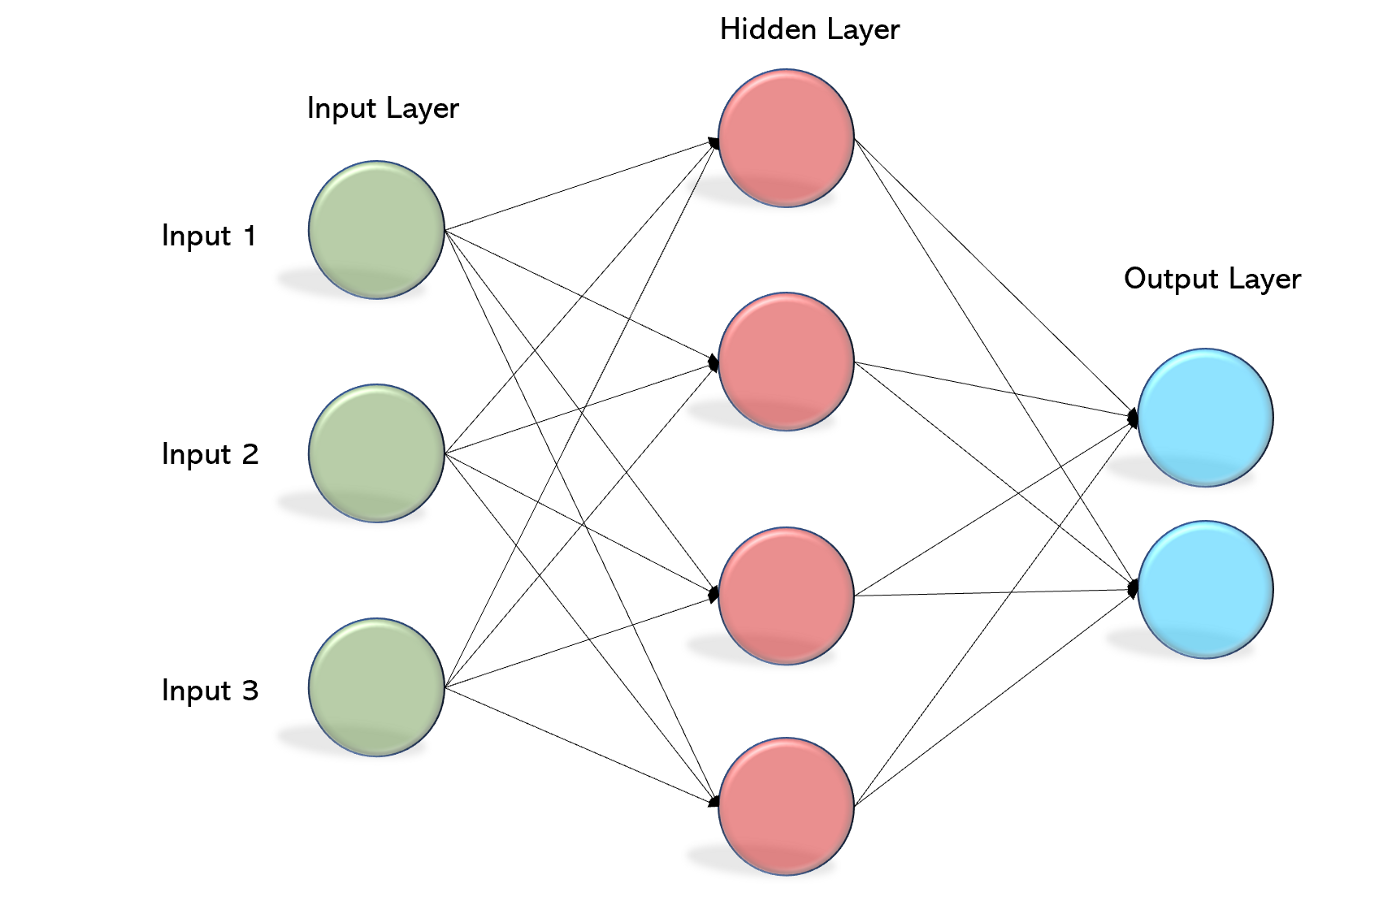
\includegraphics[width=.6\linewidth]{figures/3mlp.png}
        \caption{An example 3-layered multi-layer perceptron (MLP)}
        \label{fig:3mlp-example}
    \end{figure}

    \framebreak

    \begin{exampleblock}{Using \refann{} for SKE}
        \begin{enumerate}
            \item \alert{prune} the network's hidden units and input neurons
            \item approximate the hidden units' activation function with a \alert{2-steps-wise} linear function
            \item approximate the output units' activation function with a \alert{3- or 5-step-wise} linear function
            \item rewrite each output neuron as a \alert{linear combination} of the input neuron
            \item rewrite the linear combinations as rules
            %
            \begin{itemize}
                \item hence attaining a \alert{list of rules}
            \end{itemize}
        \end{enumerate}
    \end{exampleblock}

    \begin{figure}\centering
        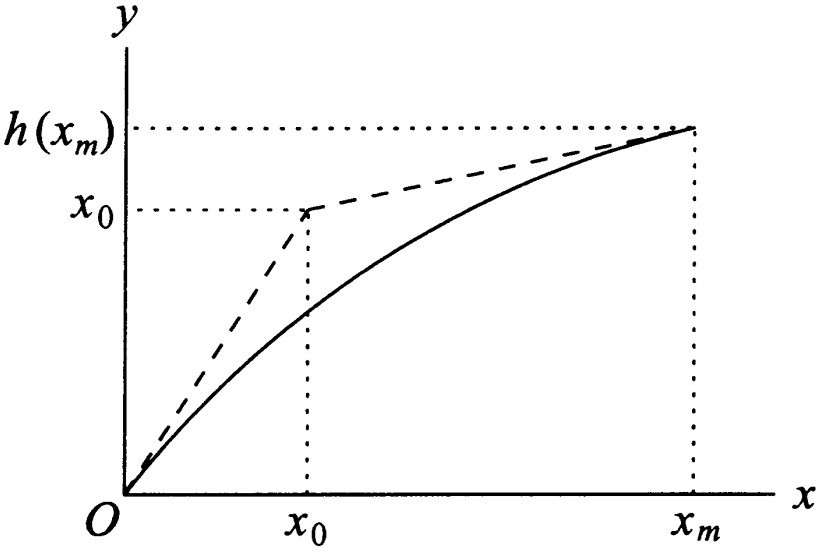
\includegraphics[width=.6\linewidth]{figures/refann/2-steps.png}
        \caption{(from \cite{setiono2002extraction}) The $tanh(x)$ function (solid curve) for $x \in [0,x_m]$ is approximated by a 2-piece linear function (dashed lines)}
    \end{figure}

    \begin{figure}\centering
        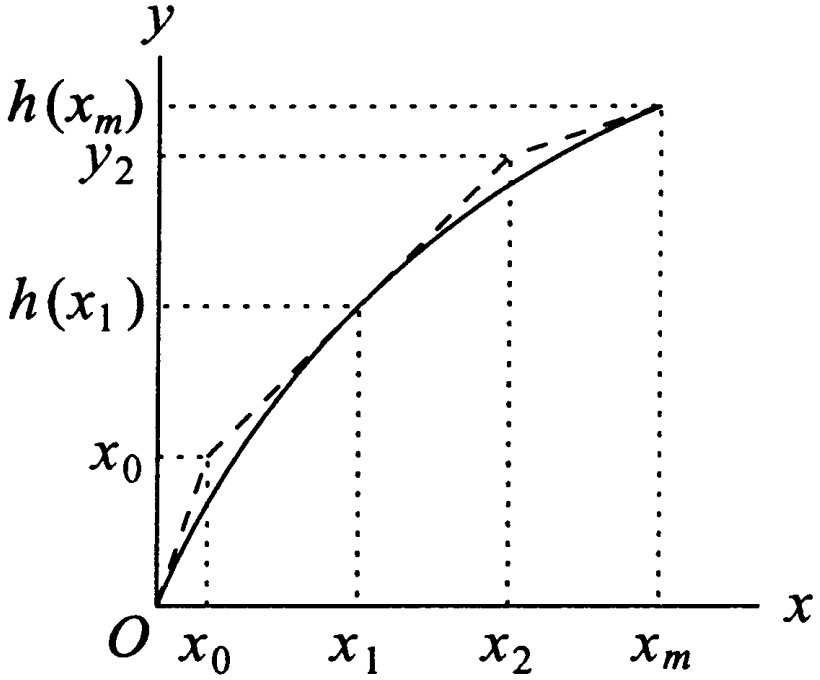
\includegraphics[width=.6\linewidth]{figures/refann/3-steps.png}
        \caption{(from \cite{setiono2002extraction}) The $tanh(x)$ function (solid curve) for $x \in [0,x_m]$ is approximated by a 3-piece linear function (dashed lines)}
    \end{figure}
    
\end{frame}

%===============================================================================
\section{A Platform for Symbolic Knowledge Extraction}
%===============================================================================

\begin{frame}[allowframebreaks]
\frametitle{Overall Design}

    \begin{center}
        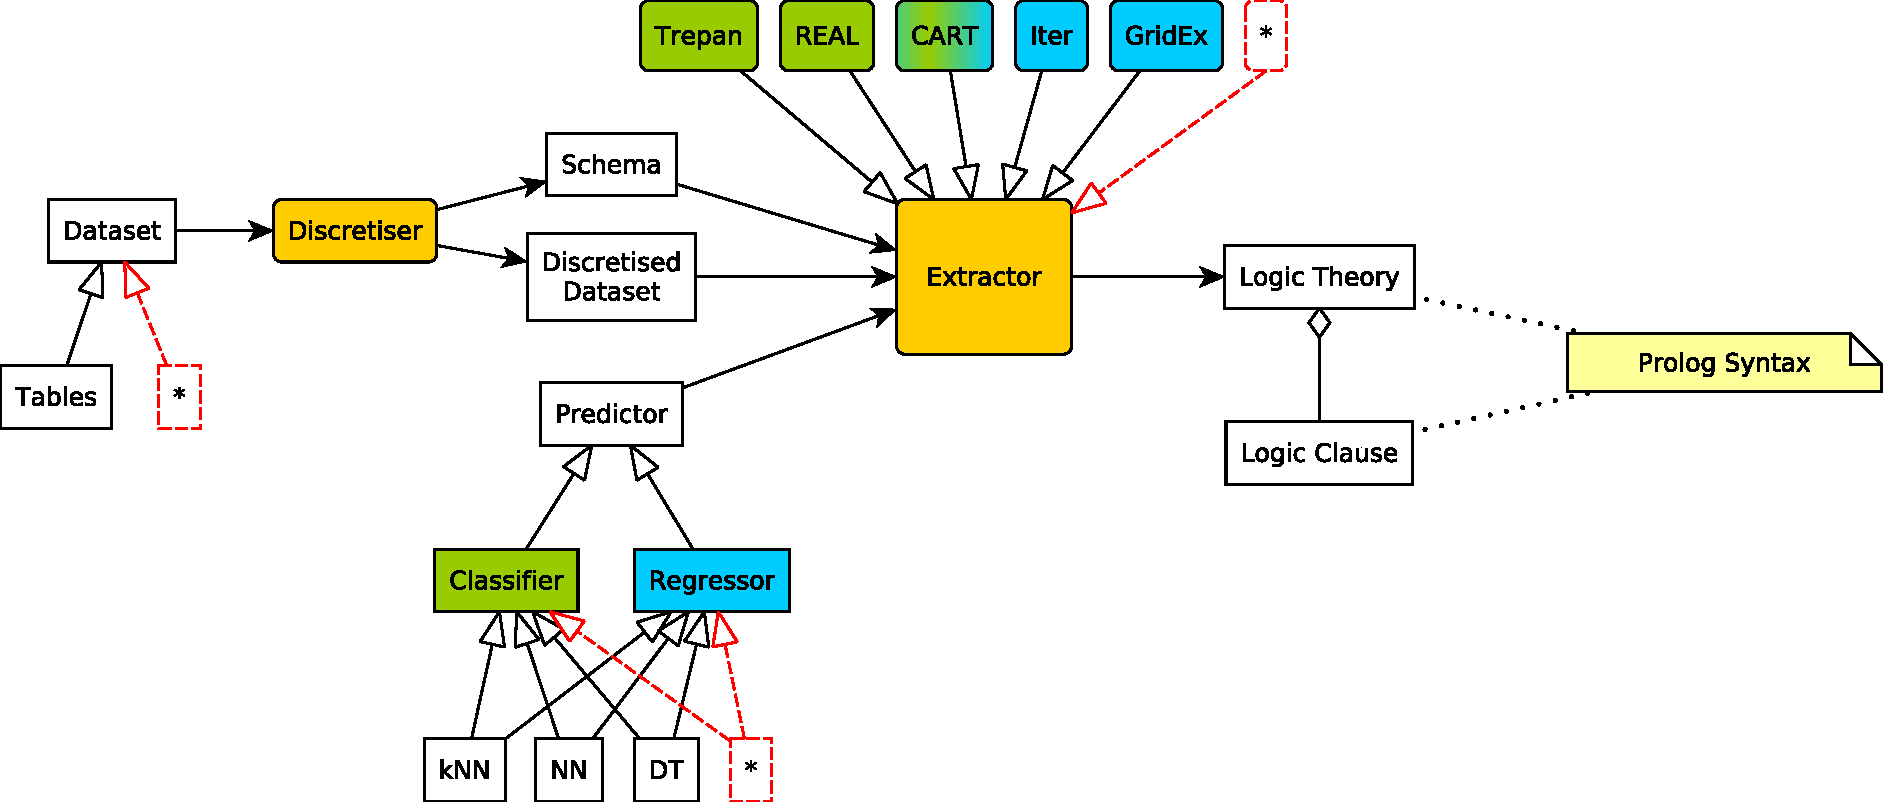
\includegraphics[width=\linewidth]{figures/Psyke.pdf}
    \end{center}

    \framebreak

    Key components:
    %
    \begin{description}
        \item[extractor:] any entity capable of extracting symbolic knowledge out of symbolic predictors
        %
        \begin{itemize}
            \item possibly, in the form of logic \alert{knowledge bases}
            \item possibly, leveraging upon the \alert{dataset} the predictor was trained upon \ldots
            %
            \begin{itemize}
                \item possibly, after a \alert{discretization} step
            \end{itemize}
            \item \ldots and its \alert{schema}
        \end{itemize}

        \item[predictor:] some trained classifier/regressor from which knowledge should be extracted
        
        \item[discretiser:] any component capable to turn continuous datasets into discrete form, following some strategy
        
        \item[logic theory:] outcome of the extraction process
    \end{description}

    \begin{block}{Unified API for SKI}
        \begin{itemize}
            \item 1 interface for \kt{Extractor}, several implementations
            %
            \begin{itemize}
                \item[eg] CART, REAL, GridEx
            \end{itemize}
            \item 1 interface for \kt{Discretiser}, several implementations
            \item 1 interface for \kt{Predictor}, several implementations
            %
            \begin{itemize}
                \item[eg] NN, kNN, DT
            \end{itemize}
        \end{itemize}
    \end{block}
\end{frame}

\begin{frame}[allowframebreaks]
\frametitle{API Design}

    \begin{center}
        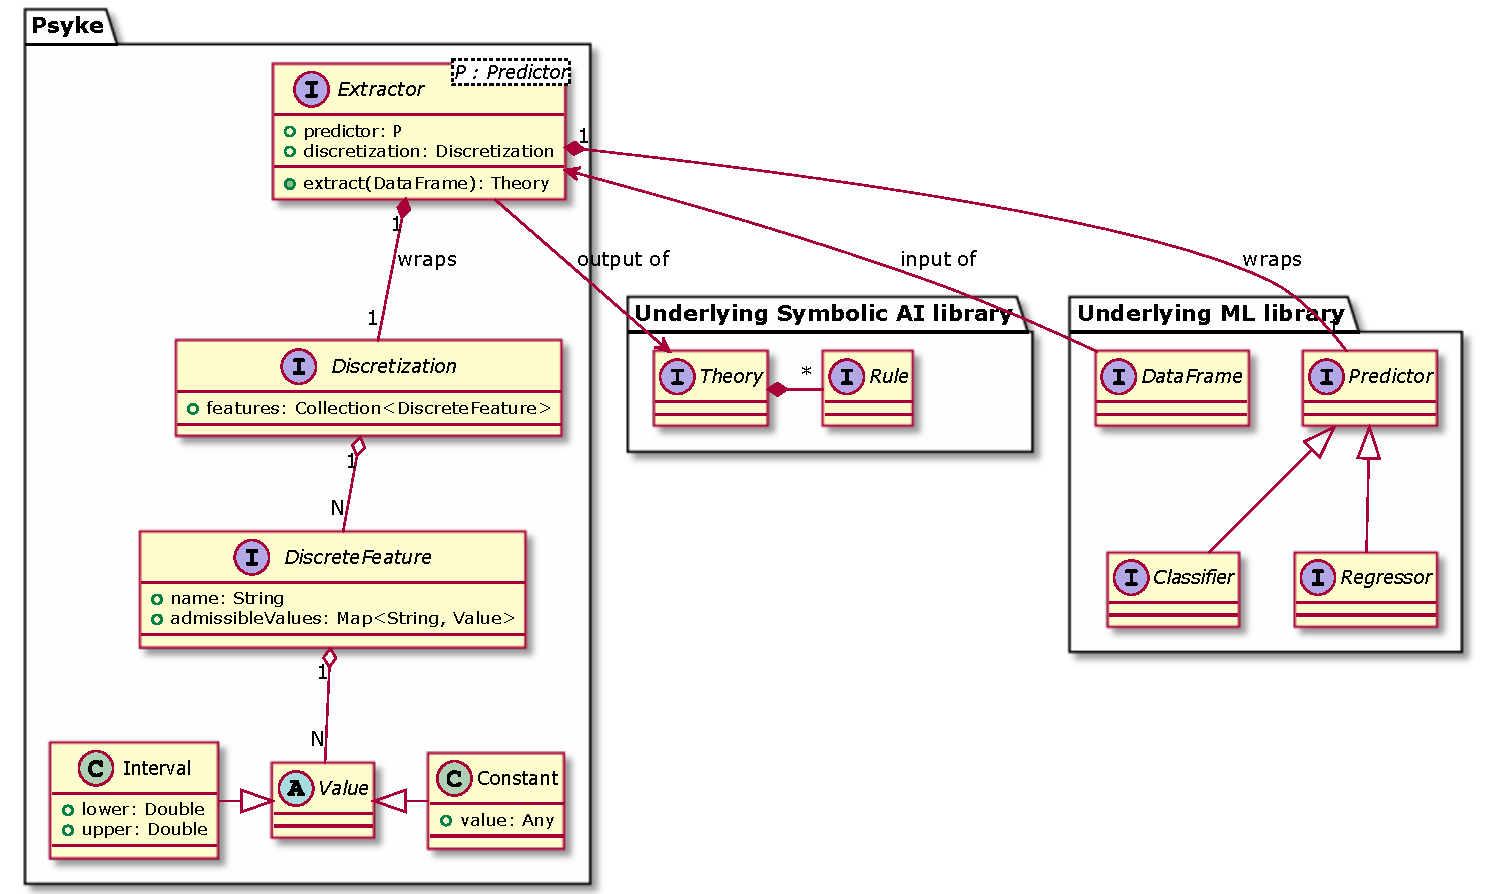
\includegraphics[width=.9\linewidth]{figures/extractor-api.pdf}
    \end{center}

    \framebreak

    General assumptions:
    %
    \begin{itemize}
        \item underlying ML library (e.g. \scikit{}\ccite{PedregosaVGMTGBPWDVPCBPD11}), providing:
        %
        \begin{description}
            \item[\kt{DataFrame}] a container of tabular data
            \item[\kt{Predictor<R>}] a computational entity which can be trained (a.k.a.\ fitted) against a \kt{DataFrame} and used to draw predictions of type \kt{R};
            \item[\kt{Classifier<R>}] a particular case of predictor where \kt{R} represents a type having a finite amount of admissible values;
            \item[\kt{Regressor<R>}] a particular case of predictor where \kt{R} represents a type having a potentially infinite (possibly continuous) amount of admissible values.
        \end{description}

        \framebreak

        \item underlying symbolic AI library (e.g. \twopkt{}\ccite{2pkt-swx16}), providing:
        %
        \begin{description}
            \item[\kt{Rule}] a semantic, intelligible representation of the function mapping \kt{Predictor}'s inputs into the corresponding outputs, for a particular portion of the input space;
            \item[\kt{Theory}] an ordered collection of rules.
        \end{description}
    \end{itemize}
\end{frame}

\begin{frame}[allowframebreaks]{About the Extracted Knowledge}

    \begin{block}{Knowledge extracted from \textbf{classifiers}}
        \begin{equation*}
            \begin{array}{rcl}
                \logicrule{\meta{task}(\var{X}_1, \ldots, \var{X}_n, \alert{\const{y}_1})}{p_{1,1}(\bar{\var{X}}),\ \ldots,\ p_{n,1}(\bar{\var{X}})}.
                \\
                \logicrule{\meta{task}(\var{X}_1, \ldots, \var{X}_n, \alert{\const{y}_2})}{p_{1,2}(\bar{\var{X}}),\ \ldots,\ p_{n,2}(\bar{\var{X}})}.
                \\
                & \vdots
                \\
                \logicrule{\meta{task}(\var{X}_1, \ldots, \var{X}_n, \alert{\const{y}_m})}{p_{1,m}(\bar{\var{X}}),\ \ldots,\ p_{n,m}(\bar{\var{X}})}.
            \end{array}
        \end{equation*}
    \end{block}

    \framebreak

    \begin{block}{Knowledge extracted from \textbf{regressors}}
        \begin{equation*}
            \begin{array}{rcl}
                \logicrule{\meta{task}(\var{X}_1, \ldots, \var{X}_n, \var{Y})}{p_{1,1}(\bar{\var{X}}),\ \ldots,\ p_{n,1}(\bar{\var{X}})},
                \\
                & & \alert{\var{Y}\ \const{is}\ f_1(\bar{\var{X}})}.
                \\
                \logicrule{\meta{task}(\var{X}_1, \ldots, \var{X}_n, \var{Y})}{p_{1,2}(\bar{\var{X}}),\ \ldots,\ p_{n,2}(\bar{\var{X}})},
                \\
                & & \alert{\var{Y}\ \const{is}\ f_2(\bar{\var{X}})}.
                \\
                & \vdots
                \\
                \logicrule{\meta{task}(\var{X}_1, \ldots, \var{X}_n, \var{Y})}{p_{1,m}(\bar{\var{X}}),\ \ldots,\ p_{n,m}(\bar{\var{X}})},
                \\
                & & \alert{\var{Y}\ \const{is}\ f_m(\bar{\var{X}})}.
            \end{array}
        \end{equation*}
    \end{block}

    \framebreak

    \ldots where:
    %
    \begin{itemize}
        \item $\mathit{task}$ is the $(n+1)$-ary relation representing the classification or regression task at hand,
        \medskip
        \item each $\var{X}_i$ is a logic variable named after the $i^\mathit{th}$ input attribute of the currently available data set,
        \medskip
        \item $\bar{\var{X}}$ is the $n$-nuple $\var{X}_1, \ldots, \var{X}_n$,
        \medskip
        \item each $p_{i,j}$ is either a $n$-ary predicate expressing some constraint about one, two or more variables, or the \pl{true} literal---which can be omitted,
        \medskip
        \item $\const{y}_i$ is the output of the $i^{th}$ prediction rule,
        \medskip
        \item $f_j$ is an $n$-ary function computing the output value for the regression task in the particular portion of the input space handled by the $j^\mathit{th}$ rule, and
        \medskip
        \item $\var{is/2}$ is the well-known Prolog predicate aimed at evaluating functions.
    \end{itemize}

    \framebreak

    \begin{block}{Underlying assumptions}
        \begin{enumerate}
            \item the input space is \alert{partitioned} into a finite set of regions

            \item each region is \alert{assigned} with a particular outcome, namely:
            %
            \begin{itemize}
                \item a \alert{class}, for \alert{classification} problems
                \item a \alert{constant}, or a simpler function, for \alert{regression} problems
            \end{itemize}

            \item \alert{one rule} generated describing \alert{for each region} and its corresponding outcome
        \end{enumerate}
    \end{block}
\end{frame}

\subsection{Usage Examples}

\begin{frame}[allowframebreaks]{Iris (classification)}\centering

    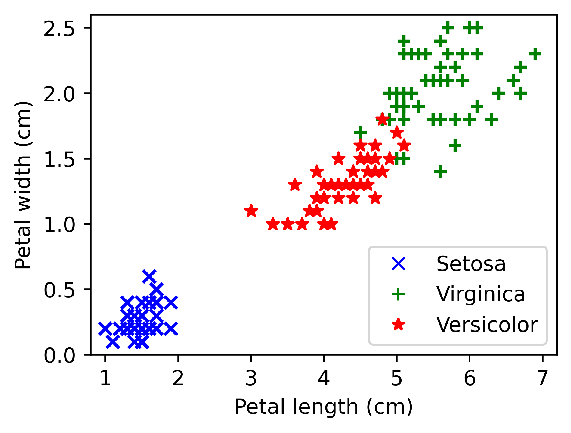
\includegraphics[width=.6\linewidth]{figures/CLA/iris-samples.pdf}

    \framebreak

    \pythonimport[basicstyle=\tiny\ttfamily]{listings/iris.py}

    \framebreak

    % !TeX root = ../ise-lab-ske.tex
\begin{figure}
    \centering

    \begin{tabular}{c|ccc}
        Predictor & \multicolumn{3}{c}{Extractor} \\
        \hline\hline
        & \real{} & \trepan{} & \cart{} \\
        \subfloat[5-NN.]{
            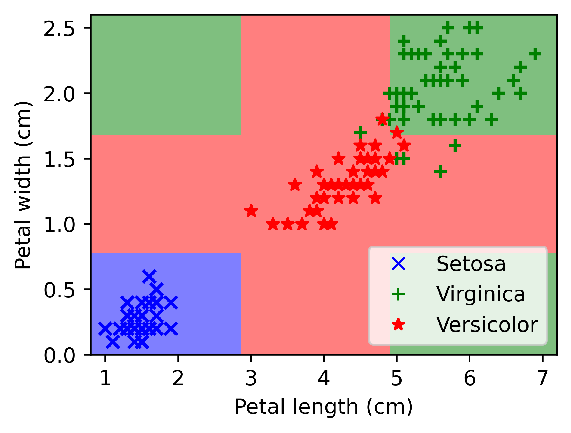
\includegraphics[width=0.20\linewidth]{figures/CLA/bb-knn.pdf}
            \label{fig:bb-knn}
        } &
        \subfloat[]{
            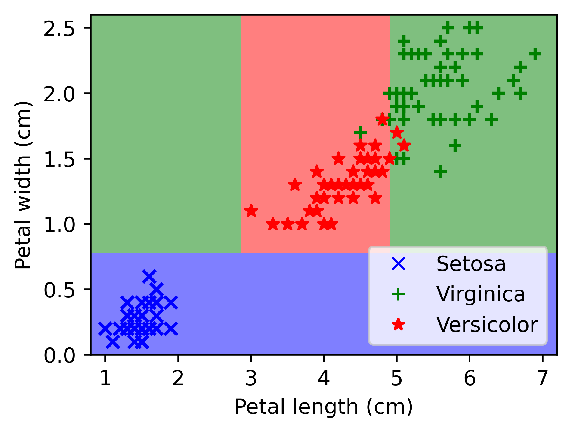
\includegraphics[width=0.20\linewidth]{figures/CLA/real-knn.pdf}
            \label{fig:real-knn}
        } &
        \subfloat[]{
            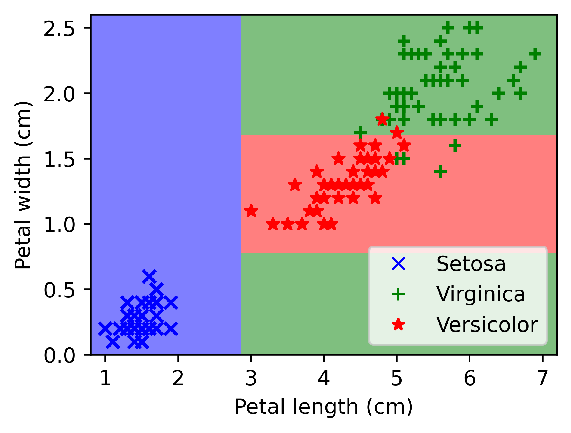
\includegraphics[width=0.20\linewidth]{figures/CLA/trepan-knn.pdf}
            \label{fig:trepan-knn}
        } &
        \subfloat[]{
            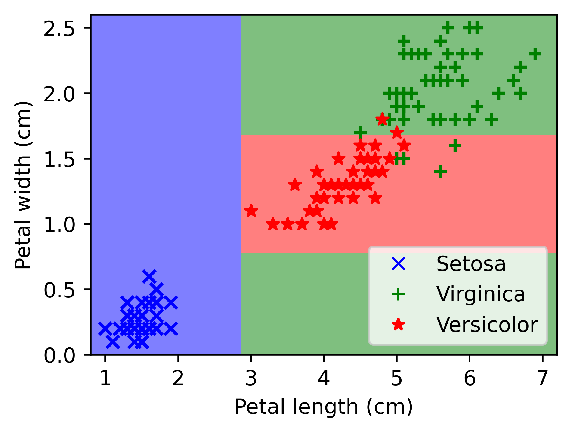
\includegraphics[width=0.20\linewidth]{figures/CLA/cart-knn.pdf}
            \label{fig:cart-knn}
        } 
        \\
        \subfloat[MLP.]{
            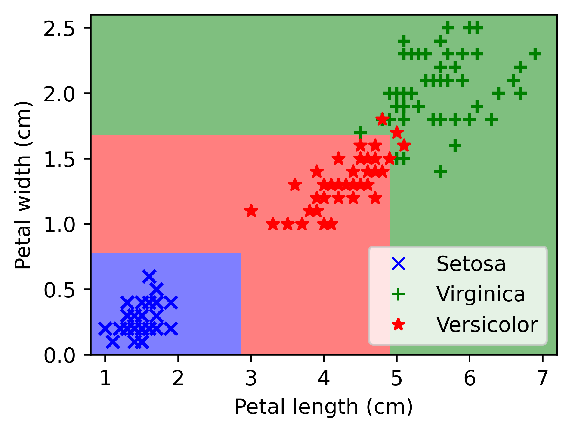
\includegraphics[width=0.20\linewidth]{figures/CLA/bb-mlp.pdf}
            \label{fig:bb-mlp-cla}
        } &
        \subfloat[]{
            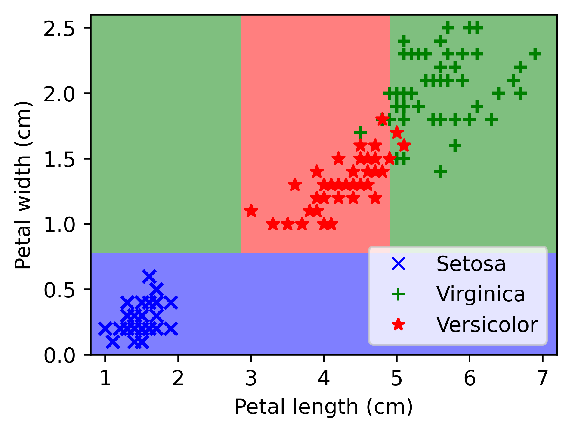
\includegraphics[width=0.20\linewidth]{figures/CLA/real-mlp.pdf}
            \label{fig:real-mlp}
        } &
        \subfloat[]{
            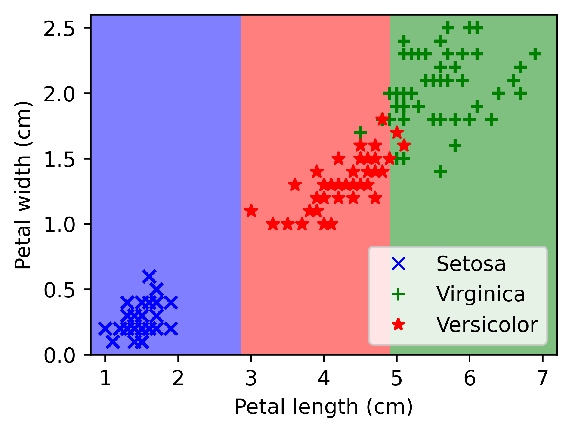
\includegraphics[width=0.20\linewidth]{figures/CLA/trepan-mlp.pdf}
            \label{fig:trepan-mlp}
        } &
        \subfloat[]{
            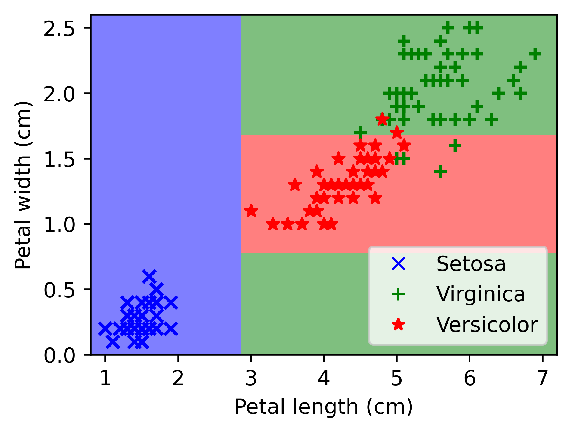
\includegraphics[width=0.20\linewidth]{figures/CLA/cart-mlp.pdf}
            \label{fig:cart-mlp-cla}
        } 			
    \end{tabular}
\end{figure}

    \framebreak

    % !TeX root = ../ise-lab-ske.tex

\begin{table}
    % \caption{Comparison between accuracy and fidelity measurements with different combinations of extraction algorithms and underlying models applied to the Iris data set}
    \begin{adjustbox}{width=\linewidth}
        \begin{tabular}{ll@{\hskip 0.8in}lll}
            \multicolumn{2}{l}{\textbf{Predictor}} & 		
            \multicolumn{3}{@{}l}{\textbf{Extractor}}\\
            \textbf{Type} & \textbf{Accuracy} & \textbf{Algorithm} & \textbf{Fidelity} & \textbf{Accuracy} \\
            \hline\hline
            5-NN & 0.94 & \real{} & 0.98 & 0.95 \\
            & & \trepan{} & 0.95 & 0.95 \\
            & & \cart{} & 0.95 & 0.95 \\
            \hline
            MLP & 0.98 & \real{} & 0.98 & 0.95 \\
            & & \trepan{} & 0.98 & 0.92 \\
            & & \cart{} & 0.98 & 0.92 \\
            % \hline
            % DT (binarised features) & 0.98 & \real{} & 0.98 & 0.97 \\
            % & & \trepan{} & 0.98 & 0.92 \\
            % & & \cart{} & 1.00 & 0.98 \\
            % \hline
            % DT (continuous features) & 0.95 & \cart{} & 1.00 & 0.95 \\
        \end{tabular}
    \end{adjustbox}
\end{table}


    \framebreak

    \prologimport[caption={Rules extracted by \real{} from MLP}]{listings/iris-real.pl}

    \framebreak 

    \prologimport[caption={Rules extracted by \real{} from 5-NN}]{listings/iris-trepan.pl}

\end{frame}

\begin{frame}[allowframebreaks]{Combined Cycle Power Plant (regression)}\centering
    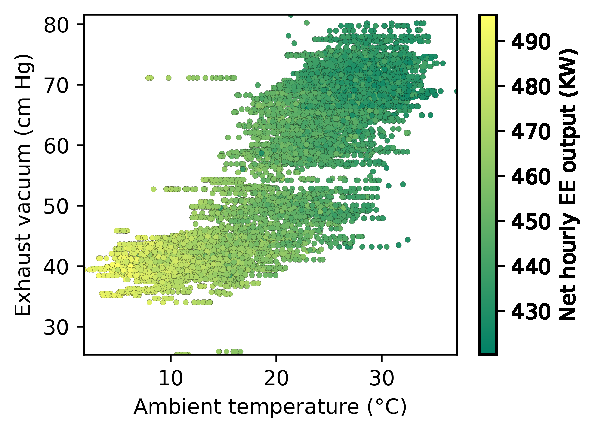
\includegraphics[width=.6\linewidth]{figures/REG/ccpp-samples.pdf}

    \framebreak

    \pythonimport[basicstyle=\tiny\ttfamily]{listings/ccpp.py}

    \framebreak

    \begin{figure}
	\centering
	\begin{tabular}{c|ccc}
		Predictor & \multicolumn{3}{c}{Extractor} \\
		\hline\hline
		& \iter{} & \gridex{} & \cart{} \\
		\subfloat[LR.]{
			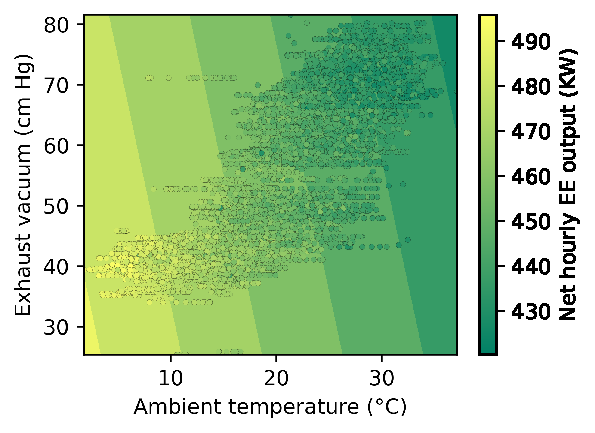
\includegraphics[width=0.215\linewidth]{figures/REG/bb-lr.pdf}
			\label{fig:bb-lr}
		} &
		\subfloat[]{
			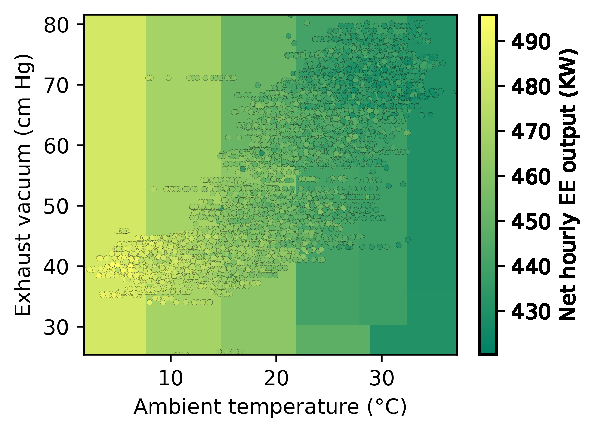
\includegraphics[width=0.2\linewidth]{figures/REG/iter-lr.pdf}
			\label{fig:iter-lr}
		} &
		\subfloat[]{
			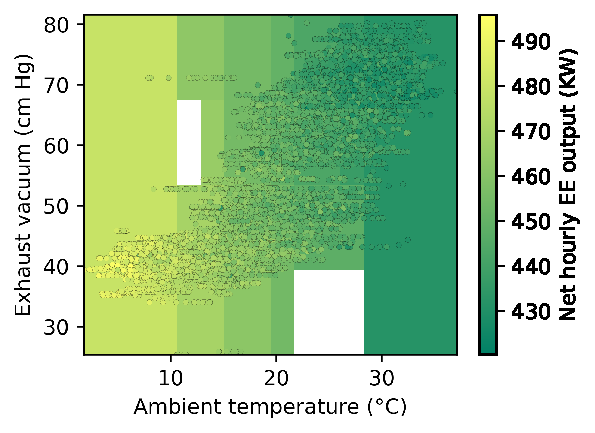
\includegraphics[width=0.2\linewidth]{figures/REG/gridex-lr.pdf}
			\label{fig:gridex-lr}
		} &
		\subfloat[]{
			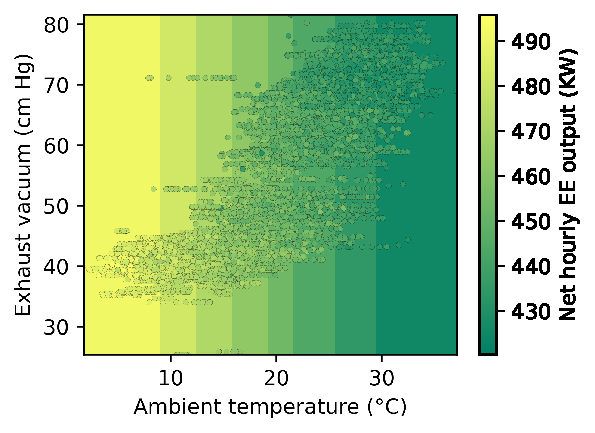
\includegraphics[width=0.2\linewidth]{figures/REG/cart-lr.pdf}
			\label{fig:cart-lr}
		} \\
		%&
		\subfloat[MLP.]{
			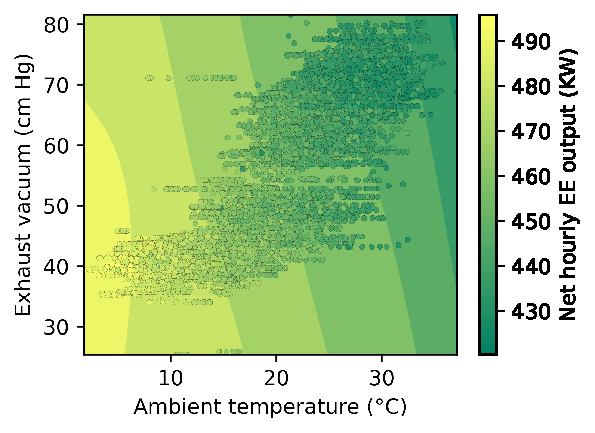
\includegraphics[width=0.2\linewidth]{figures/REG/bb-mlp.pdf}
			\label{fig:bb-mlp}
		} &
		\subfloat[]{
			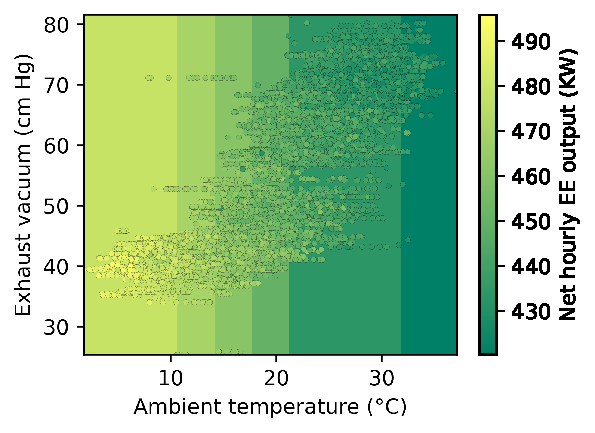
\includegraphics[width=0.2\linewidth]{figures/REG/iter-mlp.pdf}
			\label{fig:iter-mlp}
		} &
		\subfloat[]{
			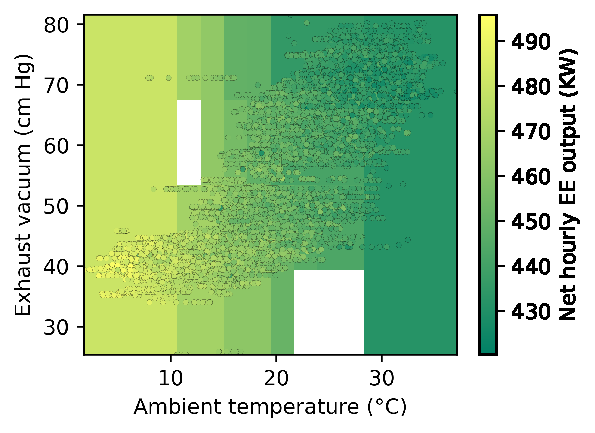
\includegraphics[width=0.2\linewidth]{figures/REG/gridex-mlp.pdf}
			\label{fig:gridex-mlp}
		} &
		\subfloat[]{
			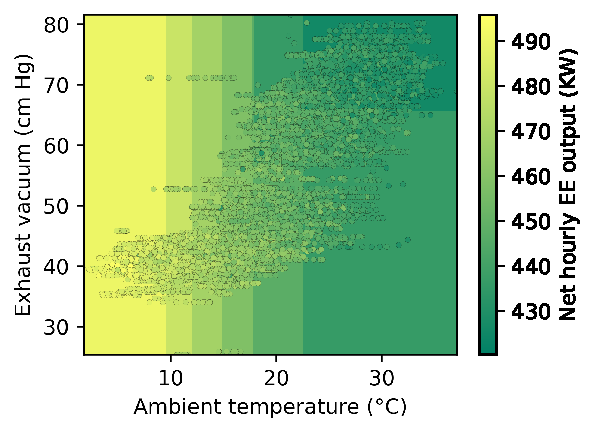
\includegraphics[width=0.2\linewidth]{figures/REG/cart-mlp.pdf}
			\label{fig:cart-mlp}
		} 
	\end{tabular}
\end{figure}

    \framebreak

    % !TeX root = ../ise-lab-ske.tex
\begin{table}
	\begin{adjustbox}{width=\linewidth}
		\begin{tabular}{lll@{\hskip 0.8in}lllll}
			\multicolumn{3}{l}{\textbf{Predictor}} & 		\multicolumn{5}{@{}l}{\textbf{Extractor}}\\
			\textbf{Type} & \textbf{MAE} & \textbf{R$^2$ score} & \textbf{Algorithm} & \textbf{MAE (data)} & \textbf{MAE (predictor)} & \textbf{R$^2$ (data)} & \textbf{R$^2$ (predictor)} \\
			\hline\hline
			LR & 3.62 & 0.93 & \iter{} & 5.47 & 4.68 & 0.84 & 0.88 \\
			& & & \gridex{} & 4.40 & 2.90 & 0.89 & 0.95 \\
			& & & \cart{} & 4.32 & 2.93 & 0.90 & 0.95 \\
			\hline
			MLP & 3.73 & 0.92 & \iter{} & 5.03 & 3.91 & 0.89 & 0.92 \\
			& & & \gridex{} & 4.40 & 2.93 & 0.89 & 0.96 \\
			& & & \cart{} & 4.25 & 2.85 & 0.90 & 0.96 \\
		\end{tabular}
	\end{adjustbox}
\end{table}


    \framebreak

    \prologimport[caption={Rules extracted for a regression problem}]{listings/ccpp-iter.pl}

\end{frame}

%===============================================================================
\section{Discussion}
%===============================================================================

\begin{frame}{Notable Remarks}
    \begin{itemize}
        \item commitment to a particular output shape / expressiveness
        %
        \begin{itemize}
            \item to preserve both human- and machine-interpretability
            \item other syntaxes may exist
        \end{itemize}
        \item discretization of the input space
        \item discretization of the output space
        \item features should have semantics per se
        \item further refinements may be applied to rules
        \item rules constitute global explanations
    \end{itemize}
\end{frame}

\begin{frame}{Current Limitations}
    \begin{itemize}
        \item tabular data as input $\rightarrow$ doesn't really work with images
        \item high dimensional datasets $\rightarrow$ very large, poorly readable rules
        \item highly variable input spaces $\rightarrow$ many rules $\rightarrow$ poor readability
    \end{itemize}
\end{frame}

\begin{frame}{Future research activities}
    \begin{itemize}
        \item target images or highly dimensional data in general
        \item target reinforcement learning (when based on NN)
        \item target unsupervised learning
        \item design and prototype your own extraction algorithm
    \end{itemize}
\end{frame}

%===============================================================================
\section*{}
%===============================================================================

%/////////
\frame{\titlepage}
%/////////

%===============================================================================
\section*{\refname}
%===============================================================================

%%%%
\setbeamertemplate{page number in head/foot}{}
%/////////
% \begin{frame}[c,noframenumbering]{\refname}
\begin{frame}[t,allowframebreaks,noframenumbering]{\refname}
%	\tiny
    \scriptsize
%	\footnotesize
    \bibliographystyle{apalike-AMS}
    \bibliography{ise-lab-ske}
\end{frame}
%/////////

%%%%%%%%%%%%%%%%%%%%%%%%%%%%%%%%%%%%%%%%%%%%%%%%%%%%%%%%%%%%%%%%%%%%%%%%%%%%%%%%
\end{document}
%%%%%%%%%%%%%%%%%%%%%%%%%%%%%%%%%%%%%%%%%%%%%%%%%%%%%%%%%%%%%%%%%%%%%%%%%%%%%%%%
